\chapter{Advanced aircraft design process: a technology review}
\markboth{Advanced aircraft design process: a technology review}{Advanced aircraft design process: a technology review}
\label{chap1:state_art}

%\begin{mdframed}[hidealllines=true,backgroundcolor=lightgray!20]
%	\section*{Résumé}
%	Ce chapitre est le premier de cette thèse et a l’objectif de présenter des notions introductives au problème.
%	Le contexte de cette recherche est lié aux défis de l’aviation pour les années à venir: la réduction des émissions est en effet un des enjeux  des clés grands sociétaux. 
%	En particulier, selon les perspectives données par Boeing et Airbus, ces deux principaux constructeurs aéronautiques estiment que plus de 20 000 appareils voleront dans les 20 prochaines années, dans le segment des courtes et moyennes distances, ce qui deviendra alors le facteur décisif pour répondre aux objectifs environnementaux.
%	Malheureusement, ces objectifs peuvent difficilement être atteints avec une configuration conventionnelle (tube-and-wing), car celle-ci est développée depuis plus de 70 ans et offre encore de faibles gains potentiels. Ainsi, un concept de rupture doit être introduit, au niveau de la conception, afin de trouver une solution prometteuse pour réduire l’empreinte environnementale de l’aviation.
%	
%	Pour mieux cerner le problème, la boucle de conception conceptuelle utilisée jusqu’à présent est détaillée.
%	Ensuite, les technologies innovantes clés étudiées au cours des dernières années sont explorées. 
%	L'innovation peut être principalement apportée à deux niveaux: modification de la cellule (géométrie) ou modification du système propulsif. En ce qui concerne la dernière catégorie, la propulsion hybride/électrique a suscité beaucoup d'intérêt: elle a été appliquée avec succès dans l’industrie automobile et les avions de petite taille et, au cours des prochaines années, différentes organisations souhaitent étendre son application au cas des avions de grande capacité. 
%	La principale caractéristique de la propulsion hybride/électrique est qu’elle permet aux nouveaux appareils de tirer parti de l’intégration entre propulsion et aérodynamique. Par exemple dans un système qui considère la propulsion électrique distribuée conjointement avec un dispositif d’ingestion de couche limite (BLI),  les effets provenant du souffle et du flux ingérant sont renforcés.
%	La discussion va plus loin: dans plusieurs ouvrages, il a été souligné que la BLI fonctionnait mieux pour des grandes cordes, ce qui met l’accent sur la recherche de l’architecture la plus appropriée pour l’intégration d’un tel système. 
%	La réponse est donnée par l’aile volante, qui intègre la charge utile et la structure et offre à la fois de grandes surfaces et un volume important pour l’attribution de sous-systèmes; de plus, elle est naturellement très efficace d’un point de vue aérodynamique.
%	
%	Sur la base de ces considérations, il a été décidé d'étudier comme configuration l’aile volante à propulsion électrique distribuée. 
%	En effet, ce concept a déjà été étudié par la NASA dans le cadre de son programme N3-X, mais leurs travaux portent principalement sur la modélisation des différentes disciplines impliquées. 
%	Dans cette recherche, l'objectif est plutôt de mettre en place une procédure pour son étude au niveau conceptuel, avec une entrée en service prévue en 2035.  
%	La question qui guide cette recherche peut être formulée comme suit: ``Comment le processus de conception avion peut-il être modifié pour l’étude d’une configuration non conventionnelle dotée d’un groupe électrogène hybride innovant?''
%	La réponse peut être exprimée en trois points:
%	\begin{itemize}
%		\item La définition de nouveaux modèles afin de prendre en compte l'impact de l'architecture innovante sur la géométrie, la structure, l'aérodynamique et l'évaluation des performances;
%		
%		\item L’application d’une approche multifidélité pour calibrer les méthodes de conception du niveau conceptuel avec des simulations plus précises;
%		
%		\item La définition d'une procédure de dimensionnement basée sur l'optimisation multidisciplinaire, en raison de sa capacité à établir un compromis tenant compte de toutes les interactions entre les disciplines, particulièrement pertinente pour les aéronefs non conventionnels.
%	\end{itemize}
%	Il est à noter que le cas test considéré introduit deux innovations clés: une au niveau de la cellule (architecture aile volante) et une autre au niveau de la propulsion (utilisation de la propulsion hybride). 
%	Afin de mieux évaluer les avantages découlant de chacun de ces deux aspects, ils ont été étudiés séparément: un aéronef conventionnel à propulsion électrique répartie est d'abord pris en compte, puis un concept d'aile volante équipé de moteurs classiques. La procédure finale provient de l'intégration de ces deux études.
%\end{mdframed}
%
%\cleardoublepage

\minitoc

\clearpage

\begin{mdframed}[hidealllines=true,backgroundcolor=purple!20]
	\section*{Outline}
	
	\begin{itemize}
		\item Aviation challenges for upcoming years are identified, specifically about the problem of emission reduction. 
		
		\item The aircraft conceptual design loop is described. 
		
		\item Different solutions to match the aviation's enviromental goals are explored, to converge towards a promising disruptive concept. 
		
		\item Research problem is stated. 
		
	\end{itemize}
\end{mdframed}

\cleardoublepage

\section{The environmental context}
\label{sec:chap1_context}
In last decades world is facing with a more and more relevant environmental crisis~\cite{bib:nasa_armd, bib:environmental_outlook_2050, bib:he_aviation_course}: CO\textsubscript{2} emission are increasing year by year, and a drastic reduction of these emissions in the upcoming years is a duty, for human sustainability. 

On this scenario, aviation plays a key role too. 
Altough its environmental footprint counts for about 2\%~\cite{bib:iata}, the increasing number of aircraft flying every day, which is doubled in 15 years~\cite{bib:airbus_global_market}, plus the more accessibility to this conveyance, make the trend growing exponentially, as shown in Fig.~\ref{fig:aviation_impact_2050}. 
\begin{figure}[!h]
	\centering
	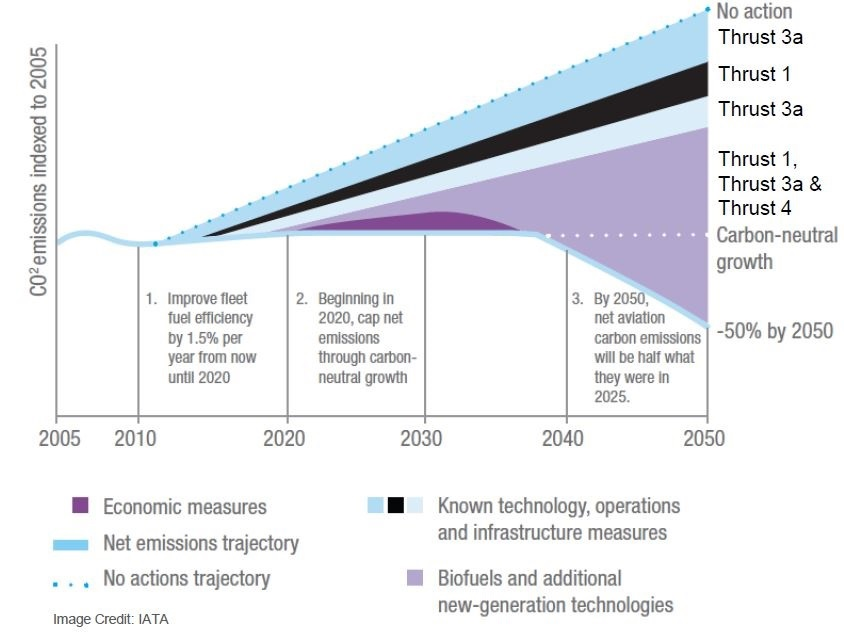
\includegraphics[keepaspectratio, width=0.6\textwidth]{images/chap1/aviation_impact_2050_perspectives.jpg}
	\caption{Aviation environmental footprint perspectives according to NASA ARMD Strategic Thrust~\cite{bib:nasa_armd}.}
	\label{fig:aviation_impact_2050}
\end{figure} 
The image, taken from the NASA ARMD Strategic Thrust~\cite{bib:nasa_armd}, shows the aviation impact perspectives in different scenarios. 
Without any action, its contribution to global emission will be soon unsustainable; the best target is to reduce CO\textsubscript{2} release up to 50\%, to maintain a sustainable level. 
The 50\% reduction goal is shared by other associations and projects in Europe too: both ATAG~\cite{bib:atag} and ACARE~\cite{bib:acare} presented their objectives, in line with the NASA studies.

According to a study, conducted by Boeing, the most critic segment is the one of large passenger aircraft (single and twin aisle)~\cite{bib:he_aviation_course}: their contribution is estimated to be around 93\%, as shown in the breakdown of Fig.~\ref{fig:aviation_emission_breakdown}.
Nowadays, with current electric technology, small regional aircraft are already being electrified, but from this analysis it is clear that the major efforts in next years will be to go on large passenger aircraft. 
\begin{figure}[!h]
	\centering
	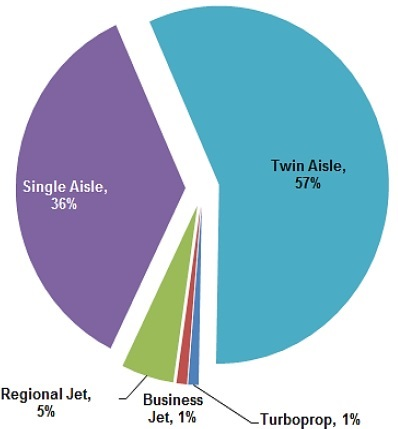
\includegraphics[keepaspectratio, width=0.4\textwidth]{images/chap1/co2_emission_breakdown.jpg}
	\caption{Percentage of CO\textsubscript{2} emission per type of aircraft~\cite{bib:he_aviation_course}.}
	\label{fig:aviation_emission_breakdown}
\end{figure} 

Besides the emissions, which remain the most important issue, also the noise and the energy consumption are relevant aspects to be reduced. 
All the goals can be summed up with a technological table, an example is given in Table~\ref{tab:nasa_armd_table}, where the short, mid and long term goals are well identified.
These are the objectives of NASA N+3 project~\cite{bib:follen_nasa_np3}, started in 2011 and still on-going: despite they seems to be very aggressive, they represent the target for the aviation's sustainability.
\begin{table}[!h]
	\centering
	\begin{tabular}{|c |c |c |c|}
		\hline
		\multirow{3}{*}{\large \textbf{Technology benefits}} & \multicolumn{3}{c|}{\textbf{Technology generations}} \\
		\cline{2-4}
		& \textbf{Near term} & \textbf{Mid term} & \textbf{Far term} \\
		& 2015--2025 & 2025--2035 & beyond 2035 \\
		\hline
		Noise & 22--32~\si{\decibel} & 32--42~\si{\decibel} & 42--52~\si{\decibel} \\
		\hline
		LTO No\textsubscript{x} emission & 70--75\% & 80\% & >80\% \\
		\hline
		Cruise NO\textsubscript{x} emission & 65--70\% & 80\% & >80\% \\
		\hline
		Aircraft fuel/energy consumption & 45--50\% & 50--60\% & 60--80\% \\
		\hline  
	\end{tabular}
	\caption{NASA ARMD Strategic Thrust table of objectives, for the subsonic transport aircraft~\cite{bib:nasa_armd}. Variation are intended with respect to 2005 best in class configuration.}
	\label{tab:nasa_armd_table}
\end{table}

To accomplish the aviation's goals, the classical tube-and-wing (TAW) configuration is not sufficient anymore: it has been developed over the last 6 decades, and it still has small potential gains. 
A disruptive configuration needs to be introduced, focusing on new and innovative configuration that features advanced technologies. 
This innovative aircraft must be introduced at conceptual design level, which is the phase of aircraft design where different configurations are studied in order to assess their performance and choose the most promising one. 
For this reason, before going through a bibliographic review about new promising technologies for future aircraft, next section will detail this phase, in order to understand how the conceptual design has been done until now. 

\section{Aircraft conceptual design cycle}
\label{sec:chap1_ac_design_cycle}

Aircraft design is a discipline over a century old and it has evolved during the years, from the first flight in 1903 to nowadays. 
Thanks to the experience gained during the decades, design methods are well assessed for a conventional \acs{TAW} architecture, and surrogate or statistical models take the place of numerical methods (\textit{i.e.} for the aerodynamics calculation)~\cite{bib:anderson, bib:raymer}.

The aircraft design process may be divided into three main steps~\cite{bib:schmollgruber_phd}: 
\begin{enumerate}
	
	\item Conceptual design phase, when a new concept is studied using reliable models, low or high fidelity according to the needs, to downselect the most promising concept.
	
	\item Preliminary design phase, where new levels of details are added to the design in order to assess the results coming from the conceptual design phase.
	
	\item Detailed design phase, where the overall configuration is well assessed and the focus is on the sizing of individual components and subsystems. 
	
\end{enumerate}
Once that the configuration is well assessed at detailed phase, a new program is launched, entering in the aircraft development. 
From now on, only conceptual design is considered, since it is the only one of interest for the research here presented. 

As listed above, the main purpose of conceptual design phase is the downselection of the most promising configuration for a given set of top level aircraft requirements (TLAR). 
This phase involves a few number of people, working for about one year. 
The rapidity is one of the main required feature in this phase, in order to analyse as many configurations as possible: for this reason, mainly low fidelity methods, \textit{i.e.} semiempirical or surrogate models, are used, but this is not a rule since when required also high fidelity methods can be employed to study a particular phenomenon~\cite{bib:mcdonald_openvsp}.
One of the reference works for the methods to use is the book series from Roskam~\cite{bib:roskam_partI}, which collects the most common methods used in the preliminary design process, still used nowaday; other milestones are the published book by Raymer~\cite{bib:raymer} and Anderson~\cite{bib:anderson}. 
Nicolai suggest to use in this phase some figures of merit, to assess the advantages of a configuration with respect to another one~\cite{bib:nicolai}.

At this stage multiple configurations can be analysed and advantages and drawbacks are discussed; after a debriefing it is possible to reduce the problem and choose a limited number of promising new configurations. 
As example, Fig.~\ref{fig:conceptual_design_example} shows all the innovative configurations studied in the first phase of the NASA N+3 project~\cite{bib:raymer_concept_design}: the benefit of each configuration has been quantified considering the estimated gain in fuel and energy reduction; at the end of the downsizing procedure the design exploration is reduced at only two promising configurations.
\begin{figure}[!h]
	\centering
	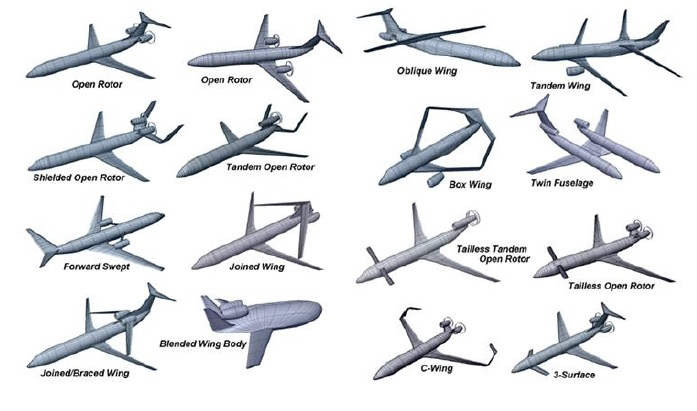
\includegraphics[keepaspectratio, width=0.6\textwidth]{images/chap1/conceptual_design_example.jpg}
	\caption{Example of possible configurations explored in the conceptual design of civil transport aircraft~\cite{bib:raymer_concept_design}.}
	\label{fig:conceptual_design_example}
\end{figure}

As first step, the constraint analysis approach is applied to define the design domain and estimate the necessary thrust~\cite{bib:roskam_partI}; on the basis of this value the engine is chosen, also considering the available technology in the foreseen EIS~\cite{bib:roskam_partII}. 
Then, weight estimation and aerodynamics can be evaluated on the basis of surrogate models, that often use few key parameters, like the wetted surfaces~\cite{bib:roskam_partV, bib:roskam_partVI}.
Performances are often evaluated on the basis of the Breguet equation~\cite{bib:anderson_perfo, bib:roskam_perfo, bib:phillips}.
More accurate methods consist in integrating the set of ordinary differential equations describing the flight dynamics~\cite{bib:roskam_flight_dynamics} using a time step integration~\cite{bib:sforza}, based on the Euler or higher degree methods like the Runge-Kutta scheme~\cite{bib:leveque_partial_equation}.

The aircraft design problem involves multiple disciplines, coupled each others (\textit{e.g.} aerodynamics provides the loads for structural sizing), and thus it may be considered as a Multidisciplinary Design Analysis (MDA).
The MDA is defined as a ``non linear system of equations obtained by the non-intuitive coupling of disciplinary solvers involved in complex engineering systems''~\cite{bib:martins_mdo, bib:gray_omdao}, specifically for this case the conceptual design problem, whereas each discipline provide a set of equations that is coupled with other disciplines.
The generic sizing procedure is given by Schmollgruber in his Ph.D. work~\cite{bib:schmollgruber_phd}; the scheme is presented in Fig.~\ref{fig:aircraft_design_xdsm}, using the \acs{xDSM} standard~\cite{bib:lambe_xdsm}.
Since this standard will be used throughout all this manuscript, it is a important to get familiar with it. 
In this notation the purple circular block represents the optimiser, meanwhile the orange one refers to a \acs{MDA} loop.
Green blocks represent the analysis, numbered according to the order of processing, and pink rectangles represent the functions.
The main workflow is identified by the black line; gray lines represent instead the data sharing.
Analyses outputs are indicated with a grey block, and finally I/O data are identified with a white block: inputs are at the top row, as outputs are at the left column.
For what it concerns the notations, $\underline{x}$ represents the design variables vector, $\underline{y}$ the state variables, apex $(0)$ indicates an initial guess, $t$ a target variable (that is, a variable that is a copy of a previous output) and $(*)$ the final value.  
Algorithm~\ref{alg:aircraft_design} reports the description of analyses, with the numbering that refers to what are used in Fig.~\ref{fig:aircraft_design_xdsm}. 
For a more detailed description refers to the already mentioned work~\cite{bib:schmollgruber_phd}.
\begin{figure}[!h]
	\centering
	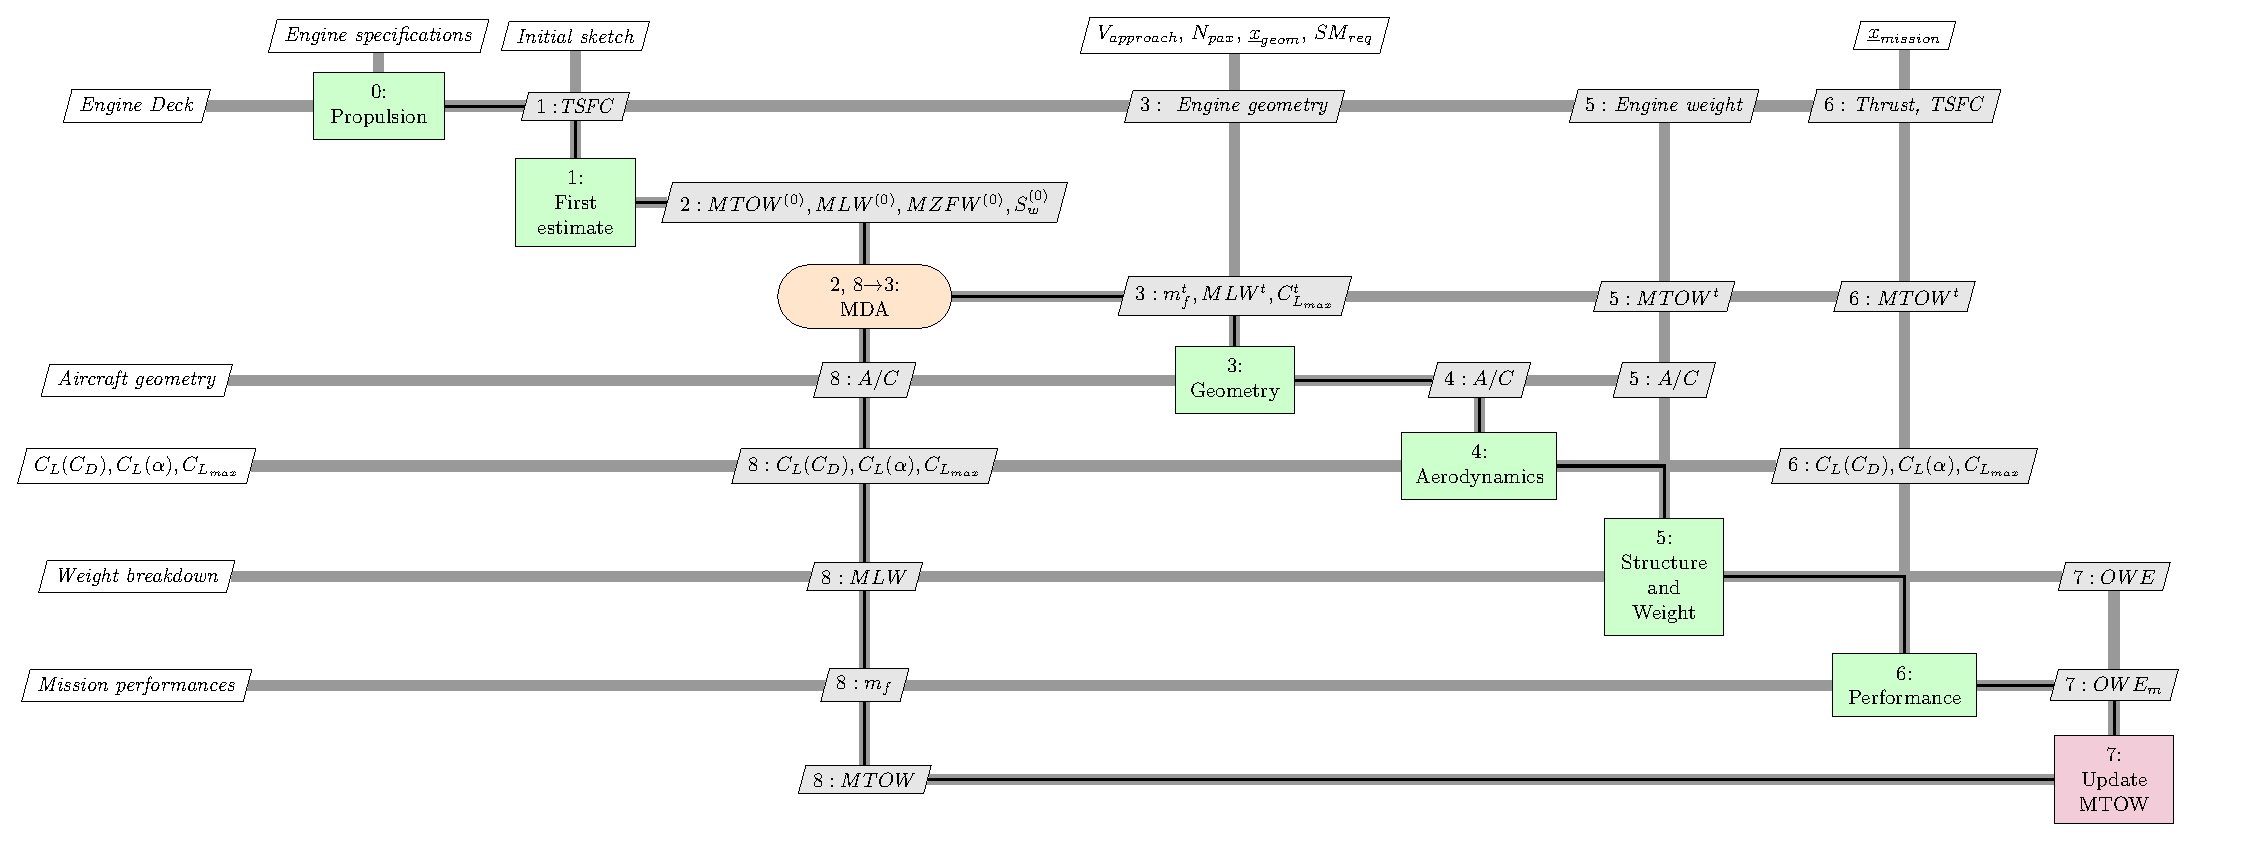
\includegraphics[keepaspectratio, width=1.2\textwidth, angle=90]{images/chap1/MDA_aircraft_design}
	\caption{Preliminary design process, using the xDSM standard presented by Lambe and Martins~\cite{bib:lambe_xdsm}.}
	\label{fig:aircraft_design_xdsm}
\end{figure}

\begin{algorithm}[!h]
	\caption{Preliminary design process algorithm. Numbering is referred to the xDSM presented in Fig.~\ref{fig:aircraft_design_xdsm}.}
	\label{alg:aircraft_design}
	\begin{algorithmic}
		\REQUIRE Initial design parameters (TLAR)
		\ENSURE Sized aircraft, drag polars, masses, design mission trajectory
		\STATE 0: Engine initialization.
		\STATE 1: Compute the initial sizing point (first estimation of wing area $S_w$, Maximum Takeoff Weight MTOW, \dots)
		\STATE 2: Initialise the loop.
		\REPEAT
		\STATE 3: Get the aircraft geometry.
		\STATE 4: Compute the aerodynamics.
		\STATE 5: Perform the structure analysis and get the weight of all the aircraft's components.
		\STATE 6: Compute performance.
		\STATE 7: Update the MTOW value.
		\STATE 8: Check the convergence: if the tolerance is below the desider thresold, return the sized aircraft, otherwise proceed to next iteration.
		\UNTIL {$8 \rightarrow 3$: MDA has converged}
	\end{algorithmic}
\end{algorithm}

In the illustrated case, engine is initialised outside the loop: one of the finding for the designers is to search for an existing engine that matches the fuel consumption targets, or to design a tailored one~\cite{bib:mattingly, bib:roux}. 
The iterative loop calls all the key disciplines involved in aircraft design: geometry, aerodynamics, structures and performance. 
Convergence is driven by the operating weight empty OWE: process is over when the value computed by structural analysis (step 5) is equal to the value computed by performance analysis (state 6).  
It must be noted that disciplines share variables, and thus are coupled each others; \textit{i.e.} structures and weight depend on the aerodynamics results, and the improvement in one of these two disciplines can lead to a degradation in the other one.
At the end more design choices can be made on the final layout, considering also the subsystems~\cite{bib:roskam_partIII, bib:roskam_partIV}. 

It is evident that the aircraft design is a matter of choosing the best compromise between the disciplines that can be considered during this phase or later (\textit{i.e.} acoustic, aeroelasticity, \dots). 
After having sized the aircraft according to given requirements, it is also worthy to study its performance on a set of operational missions, different from the design one: in general, during its life aircraft needs to supply a huge variety of missions, rarely equal to the design one~\cite{bib:roskam_partVIII}.
Tradeoff studies regarding stability or control have low priority in conceptual design phase, but can be included with very easy models, to have a first estimation before the preliminary design phase~\cite{bib:roskam_partVII}.
The Digital Datcom tool~\cite{bib:datcom} is a powerful tool to estimate stability derivatives with the help of the USAF manual~\cite{bib:datcom_ref}: data results come from statistical data on commercial aircraft and allow to size with limited approximation wing and tails~\cite{bib:sforza}. 
Despite the advantages, this tool is limited to conventional configuration, and is not reliable when the aircraft architecture differs from a TAW configuration. 

Clearly, at this point there are some uncertainties, associated to both the methods used and the perspective on the available technologies for the EIS considered; a good practice to approach this issue is through the use of some corrective factors~\cite{bib:kirby}, to assess the sensitivity with respect to technological parameters. 
The choice of the preferred configuration can be guided also by other considerations, like a preliminary cost assessment~\cite{bib:roskam_partVIII}. Once that a configuration is chosen, it is possible to proceed through the preliminary design phase, aimed to study with more detailed models to better undestand if the proposed aircraft can fulfill the customer requirements with a reasonable given cost. 

To conclude this paragraph, the conceptual design phase is well assessed for conventional configuration, but may be unable to deal with innovative concepts; however it represents the state of the art today and the starting point for future development. 

Next section reports a bibliographic review on the most promising technologies for next generation aircraft, which will be helpful in defining a promising concept to cope with environmental goals. 

\section{Key innovative aircraft technologies}
\label{sec:chap1_key_innovative_techno}

One of the \textit{leitmotiv} of aviation has always been the reduction of fuel consumption, related to emission and costs for airlines. 
For this reason, the research of innovative technologies has always been a priority in aircraft design, and with the rise of environmental constraint the works about this subject have been multiplied year by year.

Innovation can be brought at mainly two levels: architecture and propulsion~\cite{bib:isikveren_2014}. 
To the first category belong all the configurations deploying new technologies to increase the aerodynamics efficiency (expressed by the lift-to-drag ratio LoD), \textit{e.g.} the strut braced wing~\cite{bib:gur} or the active flow control~\cite{bib:iata, bib:iata_annex}.
To the second category, instead, belong the aircraft that presents innovation at propulsive level, \textit{e.g.} the Airbus Neo generation which mount high by-pass ratio (BPR) engines~\cite{bib:hughes}, or proposed concept whereas the propulsive plant has been completely modified to go towards electric/hybrid propulsion~\cite{bib:pornet_journal_he, bib:campbell_prop, bib:lambert}. 

The last case is one of the most interesting from an environmental point of view, since the possibility to employ electric source for propulsion may allow the desider emission reduction~\cite{bib:hepperle, bib:vanbogaert}.
Fostered by promising results in automotive industry, some manufacturers have already entered in the commerce with small electric aircraft; in particular it is to note the experience of Pipistrel~\cite{bib:pipistrel_alpha, bib:pipistrel_taurus} and Lange Aviation~\cite{bib:antares_main, bib:antares}. 

In practice, the challenges of designign aircraft with new propulsive systems require a cross-disciplinary effort that focuses on: feasible propulsion system, reduced fuel consumption, aviation safety and reliability, noise reduction, and optimised aircraft design to achieve desiderable performance~\cite{bib:liu_2018}. 
Starting from the very basic performance, even the Breguet equation loses its validity for this category of aircraft, and must be reformulated~\cite{bib:hepperle, bib:marwa}.
The definition of a proper powerplant is not a trivial aspect~\cite{bib:isikveren_celiner}, and also acceptance to passengers is of relevance in the introduction of such disruptive concept~\cite{bib:hornung}. 
Nevertheless, many authors, such as Freeman et al.~\cite{bib:freeman} or Seitz et al.~\cite{bib:seitz_2012}, note that new propulsive system based on hybrid/electric technologies opens new and still unexplored scenarios that may potentially be beneficial from a performance point of view. 
Campbell in its work identifies hybrid/electric propulsion as the most promising solution for revolutionary propulsion~\cite{bib:campbell_prop}.

It is to note that the electric aircraft already flying today are within the segment of small aircraft (two or four seater), whereas the most critical segment on which an action is needed is the single aisle large passenger aircraft, as shown also in the breakdown of Fig.~\ref{fig:aviation_emission_breakdown}. 
Conceptual studies to cover this segment are available in literature; next section will survey some of them to understand their impact and possible benefit. 

\subsection{Hybrid and electric propulsion technology}
\label{subsec:chap1_he_aircraft_key_techno}

This section focuses more on the concept, proposed in literature, to match the environmental goals of Table~\ref{tab:nasa_armd_table}, and thus have a long-term entry into service, except for the NASA X-57.
The study of large passenger aircraft featuring hybrid and electric (HE) propulsion has started in last decade within the NASA funded projects, as the N+3~\cite{bib:follen_nasa_np3} and the SUGAR~\cite{bib:bradley_sugar_p2, bib:bradley_sugar_p2_v2}, the Aurora D8 program~\cite{bib:aurora_d8_ref}, the PEGASUS concept~\cite{bib:pegasus}, the ECO-150 aircraft~\cite{bib:schiltgen, bib:freeman_eco150}, or the CE-Liner proposed by Bauhaus~\cite{bib:hornung, bib:steiner}, just to give some examples. 

The key aspect in these studies is the perspectives of available technologies in long-term: nowadays the exploration of the superconducting devices has started, and they show better performance than the non cryogenic technologies~\cite{bib:dever, bib:madavan}. 
The great advantage of the superconductors theory is that it eliminates the thermal management unit, which represents one of the most relevant weight penalties, and a main aspect in the sizing of electric aircraft, that can not be neglected~\cite{bib:freeman}.

Among the possibilities introduced by the hybrid/electric propulsion, two main features have been identified: distributed propulsion~\cite{bib:gohardani_book} and Boundary Layer Ingestion device~\cite{bib:smith_bli}. 
They have been noted because of their interest in terms of aero-propulsive integration and propulsive efficiency, confirmed by different authors~\cite{bib:borer_sceptor, bib:welstead_2017}, and thus they are reviewed more in detail; before going thorough these topics, some notions on hybrid/electric architecture are introduced in next paragraph. 

\subsubsection{Hybrid propulsion fundamentals}
\label{subsubsec:chap1_elec_fundamentals}

A dual-energy source aircraft can be categorised using the degree of hybridization, initially defined by Isikveren et al.~\cite{bib:isikveren}. 
The degree of hybridization is a figure of merit of the aircraft hybridization, that can be related to the power or the energy. 
It is defined as the power/energy demanded to the secondary source over the total:
\begin{subequations}
	\begin{equation}
		\label{eq:hp}
		H_P = \frac{P_{elec}}{P_{tot}}
	\end{equation}
	\begin{equation}
		\label{eq:he}
		H_E = \frac{E_{elec}}{E_{tot}}
	\end{equation}
\end{subequations}

It is to remark that the $H_P$ and $H_E$ are referred to a dual-energy source aircraft, but they do not depend by the type of sources: electric power can be delivered by batteries such as other devices, without losing any generality.
By definition, a conventional aircraft has $H_P=H_E=0$.
With the help of these definitions, four types of aircraft can be recognised, the scheme of which is shown in Fig.~\ref{fig:he_architectures}: 
\begin{itemize}
	
	\item All electric aircraft, that use exclusively electric energy and power (Fig.~\ref{fig:all_electric}).
	
	\item Turboelectric aircraft, that use combustable for energy storage but electric power to drive the propulsors (Fig.~\ref{fig:turbo_electric}).
	
	\item Series hybrid aircraft, where electrical power is supplied by the two sources that work together and are connected through an electrical node, called bus (Fig~\ref{fig:series_hybrid}).
	
	\item Parallel hybrid aircraft, where the engine provides power to propulsors mechanically. Combustion engine may use electrical power to reduce the fuel flow~\cite{bib:bradley_sugar_p2_v2}, or clutch-off to allow full electric segments~\cite{bib:ausserer} (Fig.~\ref{fig:parallel_hybrid}).
\end{itemize}

\begin{figure}[!h]
	\centering
	\begin{subfigure}{0.3\textwidth}
		\centering
		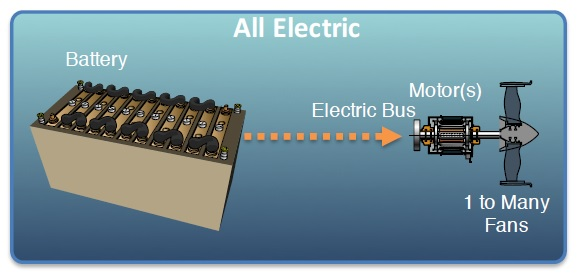
\includegraphics[width=\linewidth, height=0.15\textheight]{images/chap1/all_electric.jpg}
		\caption{All electric.}
		\label{fig:all_electric}
	\end{subfigure}
	\hspace{10mm}
	\begin{subfigure}{0.3\textwidth}
		\centering
		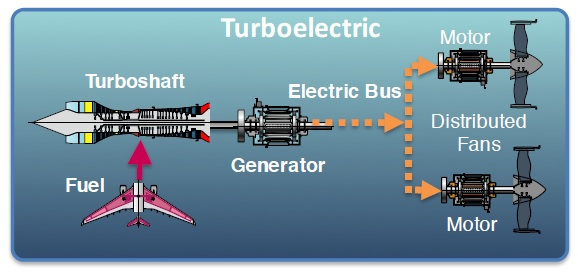
\includegraphics[width=\linewidth, height=0.15\textheight]{images/chap1/turboelectric.jpg}
		\caption{Turboelectric.}
		\label{fig:turbo_electric}
	\end{subfigure}
	\\
	\begin{subfigure}{0.3\textwidth}
		\centering
		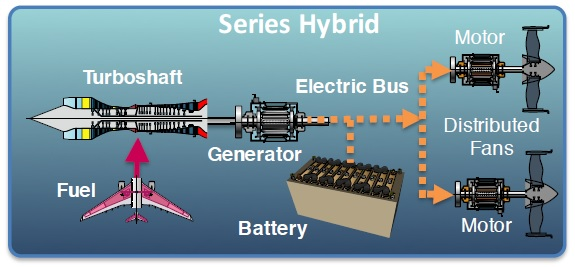
\includegraphics[width=\linewidth, height=0.15\textheight]{images/chap1/series_hybrid.jpg}
		\caption{Series hybrid.}
		\label{fig:series_hybrid}
	\end{subfigure}
	\hspace{10mm}
	\begin{subfigure}{0.3\textwidth}
		\centering
		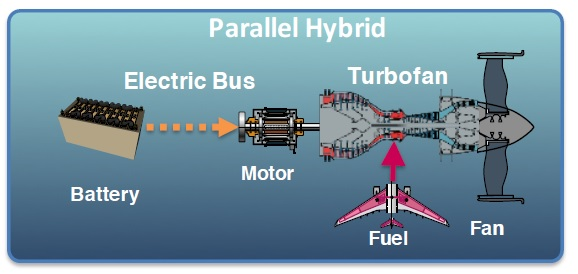
\includegraphics[width=\linewidth, height=0.15\textheight]{images/chap1/parallel_hybrid.jpg}
		\caption{Parallel hybrid.}
		\label{fig:parallel_hybrid}
	\end{subfigure}
	\caption{Different electric propulsion architectures~\cite{bib:madavan}.}
	\label{fig:he_architectures}
\end{figure}

The categories just described are classified according to the degree of hybridization as in Table~\ref{tab:he_architectures}: the classification is clear recalling the definition of $H_P$ and $H_E$.
\begin{table}[!h]
	\centering
	\begin{tabular}{l r r}
		\hline
		& $H_P$ & $H_E$ \\
		\hline
		Conventional & 0 & 0 \\
		All-electric & 1 & 1 \\
		Turboelectric & >0 & 0 \\
		Series hybrid & 1 & <1 \\
		Parallel hybrid & <1 & <1 \\
		\hline
	\end{tabular}
	\caption{Classification of electric propulsion architectures, based on the degree of hybridization.}
	\label{tab:he_architectures}
\end{table}

In an hybrid electric architecture the key points for the sizing are the power and the energy requirements: each component needs to supply a certain amount of power. 
For this reason, when evaluating this kind of concept, the two most important technological parameters, for each device, are the specific power and the specific energy~\cite{bib:fraunhofer, bib:naec}, defined respectively as the energy or the power per unit of mass. 
Specific energy content is particularly valuable for batteries design, since these elements must store a certain amount of energy, meanwhile specific power is the key design parameter for electric components that must deliver certain amount of power. 
Following the examples of Pornet et al.~\cite{bib:pornet, bib:pornet_book} and Brelje and Martins~\cite{bib:brelje_biblio}, the notation here adopted uses the lowercase to represent specific quantities of the extensive quantity: \textit{i.e.}, $e$ indicated the specific energy density and $p$ the specific power density. 

Together with the specific quantities, also the volumetric densities are relevant, since the volume available constrains the integration of the electronic systems. 
Specific and volumetric densities are related through the physical density:
\begin{subequations}
	\begin{equation}
	\rho_E = \rho e 
	\label{eq:energy_density}
	\end{equation}
	\begin{equation}
	\rho_P = \rho p
	\label{eq:power_density}
	\end{equation}
\end{subequations}
where $\rho_E$ and $\rho_P$ are the energy and power volumetric content, and $\rho$ the physical density. 

The main challenge facing HE aircraft is that batteries specific energy content is 50 times lower than that of fuel: \textit{i.e.}, for the fuel $e_f$=11900~\si{\kilo\watt\hour\per\kilogram}, meanwhile for a classical Lithium-Ion battery $e_b$=200~\si{\kilo\watt\per\kilogram}, for today's technology~\cite{bib:rheaume}.
This is also shown in Fig.~\ref{fig:energy_storage_properties}, that presents the energy characteristics for different energy storage systems. 
\begin{figure}[!h]
	\centering
	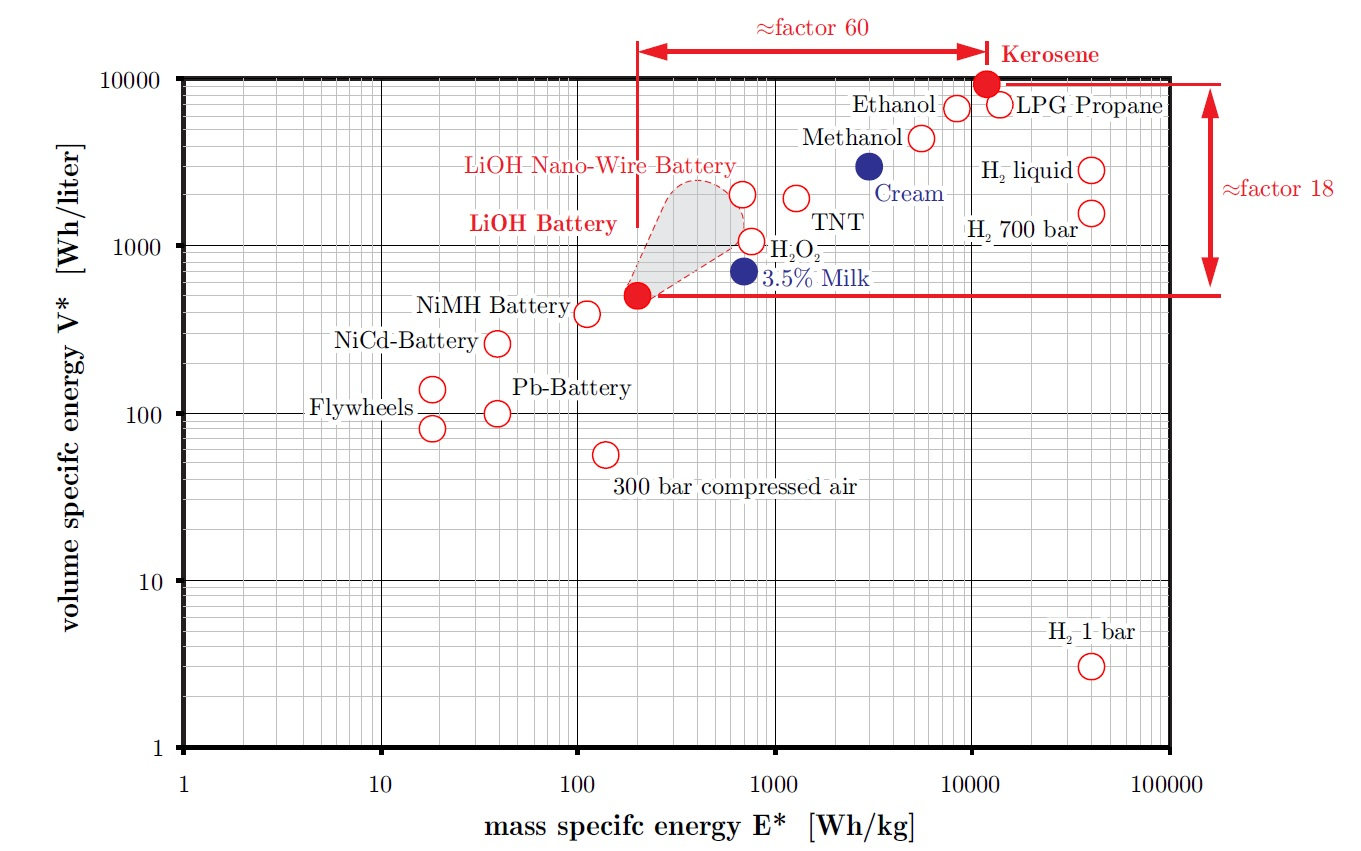
\includegraphics[width=0.8\linewidth, keepaspectratio]{images/chap1/energy_storage_properties.jpg}
	\caption{Mass specific energy vs. volume specific energy for different energy storage systems~\cite{bib:hepperle}.}
	\label{fig:energy_storage_properties}
\end{figure}

From the diagram emerges that hydrogen has a very large specific energy, even larger than the kerosene, but at standard pressure the volume content is poor, and thus it requires large volumes for the allocation. 
The problem can be avoided pressurizing the hydrogen, or using it at liquid state with a cryogenic technology, but difficulties in the identification of a sustainable production, storage and delivery system make this technology unfeasible for aviation, considering today's technological capabilities~\cite{bib:rondinelli}.

The problem of mounting and dismouting batteries' package has been addressed by Pl\"{o}tner et al.~\cite{bib:plotner} in the case of CE-Liner, and in their work they showed that integration of batteries in airframe, as well as airport operations (mounting/dismounting) do not present particular issue, for today's technology. 
Among the different types, LiOH batteries are the most perfoming, with the highest energy and volume content, that allow to have a certain amount of energy still with a feasible volume that can be mounted on aircraft.  
However, the huge difference with respect to kerosene characteristics limits the range of application: batteries introduce in fact a weight penalty, resulting in a bigger MTOW for HE aircraft. 
As a consequence, this concept is not feasible for long range distances, where the effect of carrying heavy batteries outweights the total energy advantage coming from the hybridization: its major interest is within the short and medium range segment.  

Finally, to conclude this overview on the hybrid and electric aircraft fundamentals, a metric to assess the ``goodness'' of the hybrid/electric concept must be defined.
Some of the parameters used for conventional aircraft work fine also for the hybrid electric architecture~\cite{bib:brelje_biblio}, \textit{e.g.} the fuel burn or the MTOW~\cite{bib:roskam_partVIII, bib:thorbeck}. 

Acquisition and direct costs are also relevant as metrics, specially for airlines. 
Pornet et al. preented new models for the cost evaluation, that consider the substitution of an internal combustion engine (ICE) with new hybrid power plant~\cite{bib:pornet_cost}.

Then, literature proposes other metrics: among all the possibilities, for hybrid electric aircraft are particularly relevant the energy specific air range ESAR~\cite{bib:pornet_cost, bib:ploetner} and the payload fuel energy efficiency PFEE~\cite{bib:hileman}, plus some other metrics for propulsion system performance evaluation, that prescind to the propulsive system itself and can be applied for conventional, hybrid and electric aircraft~\cite{bib:schmitz_2013}.
The ESAR quantifies the distance flown per unit of energy, and it is directly derived from the specific air range SAR (distance flown per mass of fuel). Higher the ESAR, better is the aircraft. 

The disadvantage of the ESAR, as similar metrics, is that it does not consider the payload: according to the ESAR, an aircraft that is not carrying any payload results more efficient than a loaded aircraft, when in reality the first one is not useful, since the main scope of the aircraft is to carry a certain payload from one point to another. 
To include also the useful carried weight, Hileman~\cite{bib:hileman} defined the PFEE as the range-payload per unit of energy consumed: 
\begin{equation}
	\label{eq:pfee}
	PFEE = \frac{\textrm{R} m_{PL}}{E_c}
\end{equation} 
This metric identifies an efficient aircraft as that one able to carry for longer distances a certain payload, with less energy, so it includes all the key aspects in the aircraft design. 
Unified propulsion system performance metrics proposed by Schmitz can be applied to all types of propulsion, but they do not consider the integration within the overall design and they are tailored purely to evaluate propulsive performance.
PFEE, instead, represents the most complete figure of merit to assess the validity of the hybrid concept.

\subsubsection{Distributed propulsion technology review}
\label{subsubsec:chap1_dep_review}

The distributed propulsion architecture addresses the problem of how to improve propulsive efficiency $\eta_p$.
This quantity depends on the fan pressure ratio (FPR) as follow ~\cite{bib:felder_2009}:
\begin{equation}
	\label{eq:prop_eff_fpr}
	\eta_p = 0.98 - 0.08\left(\textrm{FPR}-1\right)
\end{equation}

Engine's manufacturers have been working for years to reduce the FPR and increase $\eta_p$, but the procedure presents a relevant drawback: to keep the same thrust level, a reduced FPR requires a bigger mass flow rate passing through the fan.
This reflects on greater fan dimensions~\cite{bib:dragon}.
As example, Fig.~\ref{fig:a320_engine_comparison} shows a comparison between the engine's dimension of the A320 and its evoluted configuration, the A320Neo, mounting the new LEAP engine~\cite{bib:leap_engine}.
\begin{figure}[!h]
	\centering
	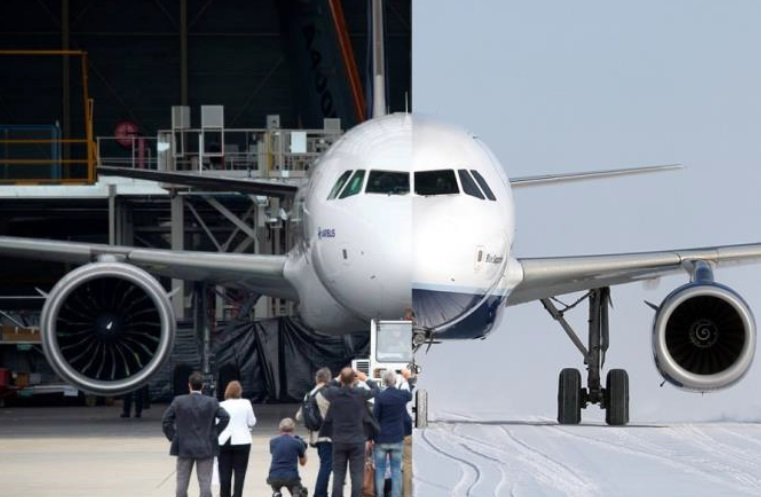
\includegraphics[keepaspectratio, width=0.6\textwidth]{images/chap1/a320_engine_comparison.jpg}
	\caption{Comparison between the Airbus A320 (right) and the new A320 Neo (left) mounting the innovative LEAP engine.}
	\label{fig:a320_engine_comparison}
\end{figure}
It is clear that it is not possible to continuously reduce the FPR, because the advantages of having a better propulsive efficiency will be counterbalanced by the augmentation in drag due to the bigger wetted surfaces. 

In this context, the distributed propulsion (DP) has a major interest, since it allows to distribute thrust on a given set of engines, with a smaller power requirement than the classical two engine configurations~\cite{bib:ko, bib:kirner, bib:dragon}. 
So with the help of DP it is still possible to reduce the FPR, keeping dimensions limited. 

As seen in previous section, the DP represents a key technology that has been massively explored in recent years.
Gohardani is one of the pioneer of the DP, and collected in a single paper all the milestones of such system, from early years to today~\cite{bib:gohardani}, and opened perspectives for its application in the electric aircraft. 
It is to underline that the DP technology is applied without considering the energy source: they can be propellers, ducted fans, moved by turboshafts or electric motors. 
Strictly speaking, this technology is related to how the total thrust can be distributed, no matter how it is produced.
To differentiate the two cases, the acronym DP is used to talk about the concept, as DEP (distributed electric propulsion) is linked with the particular application of DP to electric propulsion. 

One of the main example of DEP application to improve the propulsive efficiency is provided by DRAGON, a concept presented by ONERA~\cite{bib:dragon} and shown in Fig.~\ref{fig:dragon}. 
\begin{figure}[h!]
	\centering
	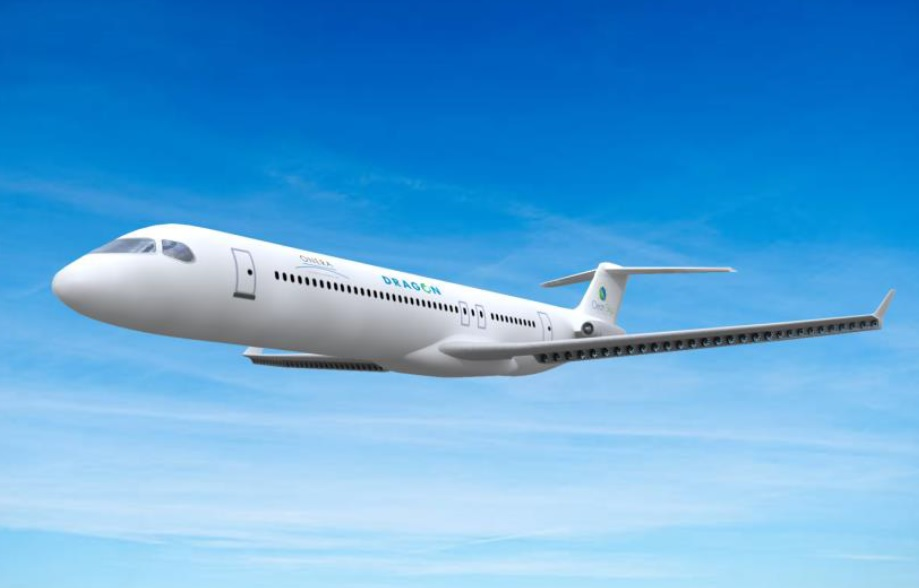
\includegraphics[keepaspectratio, width=0.5\linewidth]{images/chap1/dragon.jpg}
	\caption{DRAGON concept, proposed by ONERA~\cite{bib:dragon}.}
	\label{fig:dragon}
\end{figure}
In this concept two turboshafts provide electric power to the motors, mounted on the wing lower surface.
This concept is represented of the downsizing due to the distributed propulsion, and represents a practical application of DEP applied to the segment of major interest in this research. 
Tradeoff studies on this configuration are promising and identify potential gains with respect to reference conventional aircraft.
Also, this work addresses the problem of the mass variation due to the presence of a distributed propulsion system: in theory, the distributed weight along the wing relax the bending moment at the wing root, resulting in a possible less stiffened structure. 
In practice, the authors explain that this analysis does not include the torsion moment generated by the engines, and some preliminary analyses show that the final weight finally results increases~\cite{bib:dragon}. 
Kim et al. further developed the propulsive and weight aspects, adding some knowledge to the aforementioned work of Gohardany~\cite{bib:kim_dep, bib:kim_dep_review}: they proposed a benchmark of typical weights and aircraft parameters featuring DEP. 

Moreover, the potentiality introduced by DEP are not only limited to a better propulsive efficiency: indeed, the idea is 60 years old and dates back to 1924, when Manzel considered the possibility of distributing propellers over a row~\cite{bib:manzel}.
He had an intuition that in this system aerodynamics and propulsive aspects are correlated; in some experimental work he detected that the region interested by the presence of distributed fan is subject to a blowing, which energizes the fuel. 
In this condition it is possible to potentially have laminar flow with increased lift, resulting in a reduced takeoff and landing length; unfortunately the project has been abandoned for lack of knowledge. 
His idea was further developed at the beginning of the VTOL concepts~\cite{bib:malvestuto}, and it has been further developed up to today; even the basic idea was the same of Manzel, his concept has been brought on a new level, thanks to the knowledge gained in over 80 years~\cite{bib:gohardani_book}. 

The state of the art for the DP application is the NASA SCEPTOR X-57 demonstrator~\cite{bib:borer_sceptor} shown in Fig.~\ref{fig:nasa_x57}. 
\begin{figure}[h!]
	\centering
	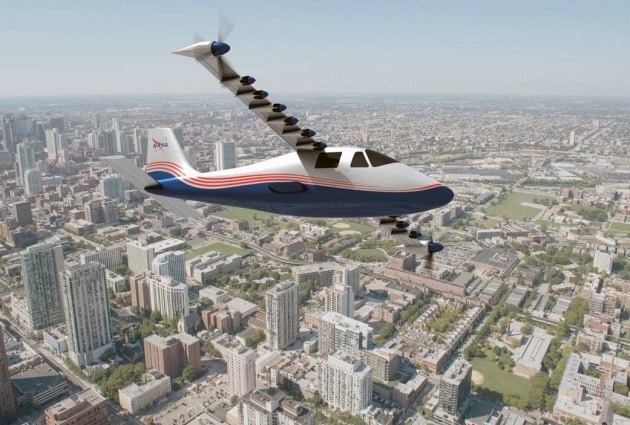
\includegraphics[keepaspectratio, width=0.5\linewidth]{images/chap1/nasa_x57.jpg}
	\caption{NASA SCEPTOR X-57 concept~\cite{bib:borer_sceptor}.}
	\label{fig:nasa_x57}
\end{figure}
It is a small aircraft, based on the existing Tecnam P2006T aircraft, that proposes to use two wingtip propellers, to reduce induced drag, and a certain number of smaller distributed propellers, to take advantages of distributed propulsion through the blowing effect to increase the maximum $C_L$~\cite{bib:deere_2017b}. 
High-lift devices are not needed anymore, leading to an easier and lighter wing structure; however, the distributed propellers require an accurate wing design~\cite{bib:deere_2017a}. 
To avoid problem in cruise, where the blowing worsenes the handling qualities, the small propellers are used only for takeoff and landing, then they are flapped and only the two wingtip propellers are used. 
The electric version of the NASA X-57, sometimes referred as NASA X-57 Maxwell, mounts Lithium-Ion batteries to supply electric power. 
Thermal~\cite{bib:schnulo} and control aspects~\cite{bib:clarke} of this configuration have been studied, then the batteries and the propellers have been optimised with respect to the mission requirements~\cite{bib:hwang_x57}: it is possible to say that the work on the NASA X-57 is the most comprehensive and represents the best example of electric integration benefits. 
It is also a milestone in the distributed propulsion effects on performance and sizing~\cite{bib:moore_2018}. 

Another interesting concept, in the same segment as the X-57, is AMPERE~\cite{bib:ampere_ref}, developed at ONERA and depicted in Fig.~\ref{fig:ampere}. 
\begin{figure}[h!]
	\centering
	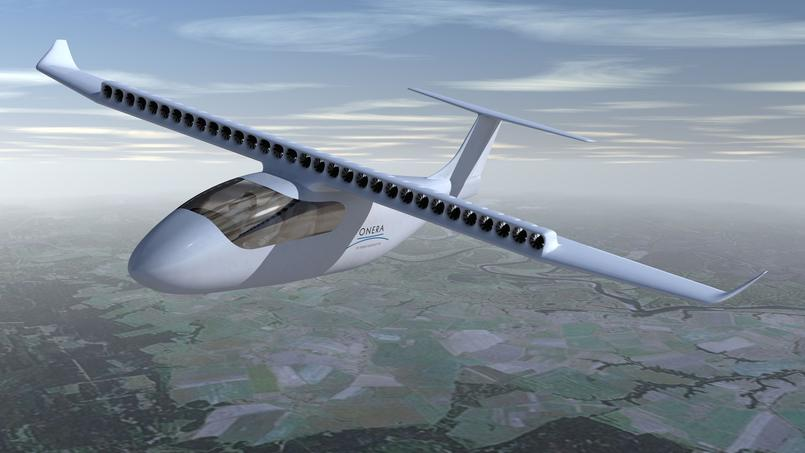
\includegraphics[keepaspectratio, width=0.5\linewidth]{images/chap1/ampere.jpg}
	\caption{AMPERE concept, proposed by ONERA~\cite{bib:ampere_ref}.}
	\label{fig:ampere}
\end{figure}
Instead of having distributed propellers, the propulsion is obtained with a set of ducted fans, distributed along the wing. 
Differently from the previous example, the blowing effect is acting in all the mission phases, and thus to understand how it impacts on the handling qualities wing tunnel tests and simulations have been carried out~\cite{bib:dillinger_ampere}. 

Nevertheless, blowing phenomenon is just one of the aerodynamics effects introduced by DP: Manzel already mentioned the possibility of a laminar flow over the wing, and in recent years Borer et al.~\cite{bib:borer}, for the case of NASA X-57, showed that indeed laminarity is obtained and assessed the related aerodynamics improvement. 
Hovewer, the benefits strongly depend on the engines' position: Wick et al.~\cite{bib:wick} considered three different configurations, with engines over the wing, integrated within the structure and under the wing, and it has been seen that the aerodynamics strongly depends on how the engines are distributed. 
The embedded configurations are even harder to analyse, due to the strong coupling between the aerodynamics and the propulsion, as well as the structural side of building wing with propulsors integrated in the airframe~\cite{bib:khero}. 
Hoogref et al.~\cite{bib:hoogreef}, on the contrary, concluded showing that the DP must be rediscussed, because the advantages can not be so marked as the literature may suggest.
At this stage, further analyses have to be conducted to select the most promising disposition to benefit of DP. 

Another non trivial feature of DP is linked to the possibility of engines downsizing. 
Generally, one of the main requirements to meet in aircraft design is the case of one engine inoperative (OEI)~\cite{bib:roskam_partI}.
This condition in a DP system becomes less stringent: in fact, in case one engine is out, to get the same thrust level the other engines must provide less thrust \textit{i.e.} in case of 4 engines deployed than 2~\cite{bib:steiner}. 
This concept is better illustrated in Fig.~\ref{fig:oei_condition}.   
\begin{figure}[h!]
	\centering
	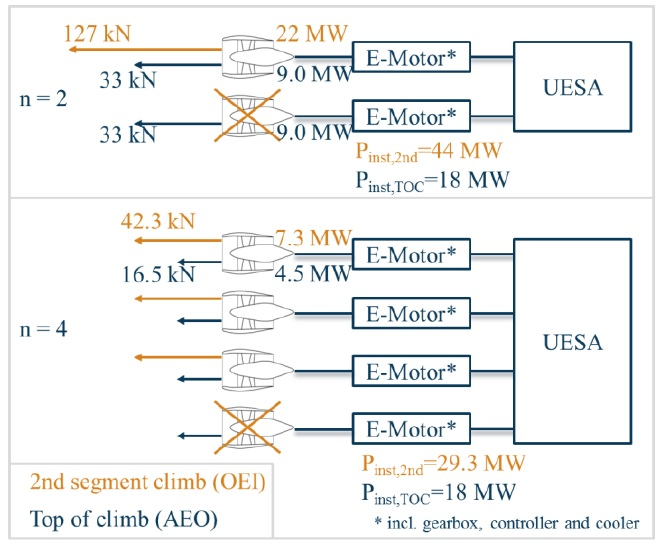
\includegraphics[keepaspectratio, width=0.5\linewidth]{images/chap1/oei_condition.jpg}
	\caption{Illustration showing the difference in the engine sizing to meet the OEI condition for 2 and 4 motors~\cite{bib:steiner}.}
	\label{fig:oei_condition}
\end{figure}
Of course, a lower installed thrust is directly linked to a smaller engines; it is to mention that on a safety point of view the DP may be considered safer than the classical one, since it intrinsecaly adds redundancy. 

Safety aspects of the DP are treated by Papathakis et al.~\cite{bib:papathakis}, but so far a full comprehension of all the issues related to security is still a remarkable challenge.
At this stage, research is still far to define a preferrable arrangement for the engines, to maximise aerodynamics' benefit; also, due to the strong integration between different disciplines, so far the works are limited by the use of high fidelity tools, and thus the DP effects in the overall design process have not been considered yet. 
A clear and shared DP terminology is desiderable in the future to permit to better discuss this emerging technology.
Then, more detailed studies are needed to identify an optimised framework, involving weight, number of propulsion units, and other top level aircraft parameters, to meet a commercial configuration capable to go through a sustainable civil aviation. 

Distributed electric propulsion is only one of the two features identified for hybrid/electric technology, the other one is the BLI, which enhances the advantages of DEP and viceversa, as it will be better detailed in the following section. 

\subsubsection{Boundary layer ingestion device}
\label{subsubsec:chap1_bli_review}

The second aspect identified for hybrid and electric configurations is the Boundary Layer Ingestion (BLI) device: it is one of the core technologies that may impact the distributed propulsion technology.
The BLI idea arose at the beginning for marine applications~\cite{bib:park, bib:roberts} and has been lately applied to aircraft~\cite{bib:tournier, bib:owen, bib:allan, bib:peijian}, mainly in subsonic configurations, but some examples on supersonic jet can be found too~\cite{bib:kumar}.

A non negligeable part of the total drag around a body in a flow comes from the boundary layer~\cite{bib:monti_pt2}; the BLI is a device that reduces this contribution by partially ingestion the boundary layer~\cite{bib:smith}. 
As for the DEP, this technology is not recent: one of the early application comes from the work of Smith and Roberts~\cite{bib:smith_bli} in 1947.
In their work, they compared a conventional turbojet configuration with one having installed boundary layer suction devices within some slots in the wing. 
They assessed a 30\% improvement in fuel efficiency and a 7\% higher optimum cruise speed due to the suction of the boundary layer; also they demonstrated that BLI increases the lift-to-drag ratio, reduces takeoff length and contributes to enhance control characteristics. 
Again, its development has been stopped because of lack of knowledge needed, but the improvement since then allows to consider such device for today's applications.

The main challenge in dealing with the BLI lies in a proper formulation to assess the benefits: since it includes the boundary layer aspects, a fully RANS model needs to be used. 
The most important phenomenon related to BLI is that the flow field results changed: streamlines are not parallel to the body anymore and distorsion occures at the inlet entrance. 
Considering only this effect may result limiting in the evaluation of the BLI benefits; Plas et al.~\cite{bib:plas} report all the physical phenomena that occur in BLI and need to be considered: 
\begin{itemize}
	\item State of the boundary layer coming into the intake;
	\item Inlet design, both outside and inside;
	\item Evolution of the non-uniform inlet flow from intake entrance to engine face;
	\item Distorsion transfer across the fan;
	\item Response of the fan to the distortion, which may impact operability and aeromechanics;
	\item Evolution of the flow downstream of the fan;
	\item Duct losses, which shows an high sensitivity because of low FPR; 
	\item Potential flow separation and unsteadiness of the flow field. 
\end{itemize}

So far, the most common way to treat the BLI is with the help of a RANS model: Gray et al. presented an approach in which these equations are coupled with the propulsion, and the geometry is optimised to maximize the benefits of the BLI in the STARC-ABL concept~\cite{bib:gray}.
The same authors optimised the overall turboelectric propulsion system featuring the BLI~\cite{bib:gray_bli_2018}. 
NASA presented an easier modellisation, yet using high fidelity, based on the entropy calculation and successfully used in the N+3 concept studies~\cite{bib:bwb_n3_vol1, bib:bwb_n3_vol2}; ONERA reported a similar approach, but based on the exergy more than the entropy~\cite{bib:arntz}. 
De la Rosa Blanco et al. considered the BLI as basis for a silent aircraft engine, noting the advantages in noise reduction; they also assessed a gain of about 4\% with respect to the best in class with the BLI~\cite{bib:silent_engine_aircraft}. 
There is no evidence of surrogate models, or semi-empirical equations, capable to deal with this phenomenon at low fidelity, and this may be understandable because of the large number of phenomena to be considered. 

Another issue is the definition of a figure of merit to evaluate performance; different authors use the power saving coefficient PSC, defined as below~\cite{bib:smith}:
\begin{equation}
	\label{eq:psc_bli}
	\textrm{PSC} = \frac{P_{ref}-P_{BLI}}{P_{ref}}
\end{equation}

In the equation above, $P_{ref}$ is the reference power of a non-BLI propulsor and $P_{BLI}$ the power required by the propulsors in case the BLI is mounted: as such, PSC quantifies the reduction in the power needed, on a common configuration, with and without the boundary layer suction. 
It is clear that the BLI represents a key feature and may be beneficial for the emission' reduction, despite the huge number of challenges that it poses. 

The most interesting application of BLI is the STARC-ABL~\cite{bib:welstead_2016}, shown in Fig.~\ref{fig:starc_abl}. 
This concept was born because the NASA wanted to develop a concept feasible in the nearer term, overcoming the high technological barrier set by N+3 program~\cite{bib:bradley_sugar_p2_v2}. 
\begin{figure}[!h]
	\centering
	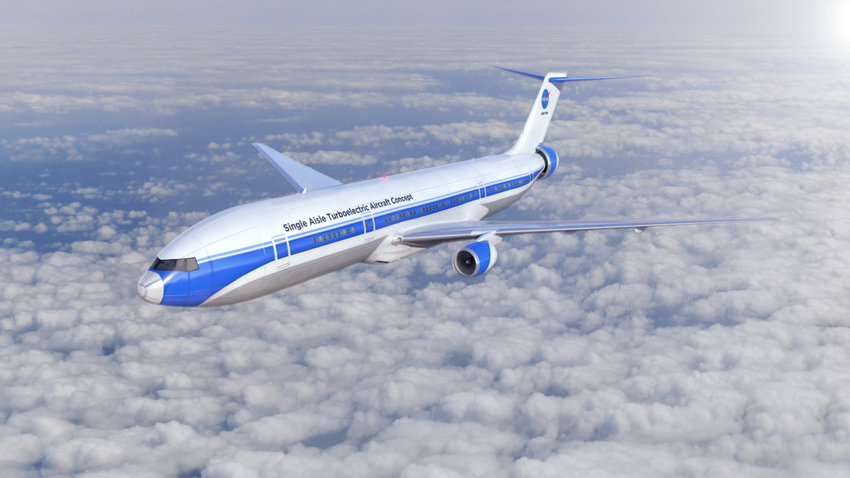
\includegraphics[keepaspectratio, width=0.6\textwidth]{images/chap1/starc_abl.jpg}
	\caption{STARC-ABL concept, proposed by NASA~\cite{bib:welstead_2016}.}
	\label{fig:starc_abl}
\end{figure}
In the STARC-ABL a tailcone propulsor is mounted on a conventional \acs{TAW} fuselage, and it works coupled with two downsized turboshafts, which provide power needed~\cite{bib:yoon}.
The tail-cone propulsor is integrated within the fuselage and mounts a BLI device, capable to ingest around 60\% of the fuselage boundary layer~\cite{bib:welstead_2017}. 
The performance assessment shows a 10-12\% fuel burn reduction thanks to the BLI. 
Another interesting study concerns the dynamic behaviour of the propulsive system, analysed in one of the latest work on STARC-ABL~\cite{bib:kratz}: the dynamic of electric system is indeed an aspect that cannot be neglected during the design of powerplant components; but the level of detail is already higher than that required at conceptual design. 
The program is still active and more studies are foreseen in the next years.

On European side, the CENTRELINE consortium is investigating a concept similar to the STARC-ABL, with propulsive fuselage, called CENTRELINE~\cite{bib:seitz_2018, bib:habermann_2018, bib:bijewitz, bib:goraj}.
The aircraft is depicted in Fig.~\ref{fig:centreline}; an entry into service 2035 is foreseen for the concept.  
\begin{figure}[!h]
	\centering
	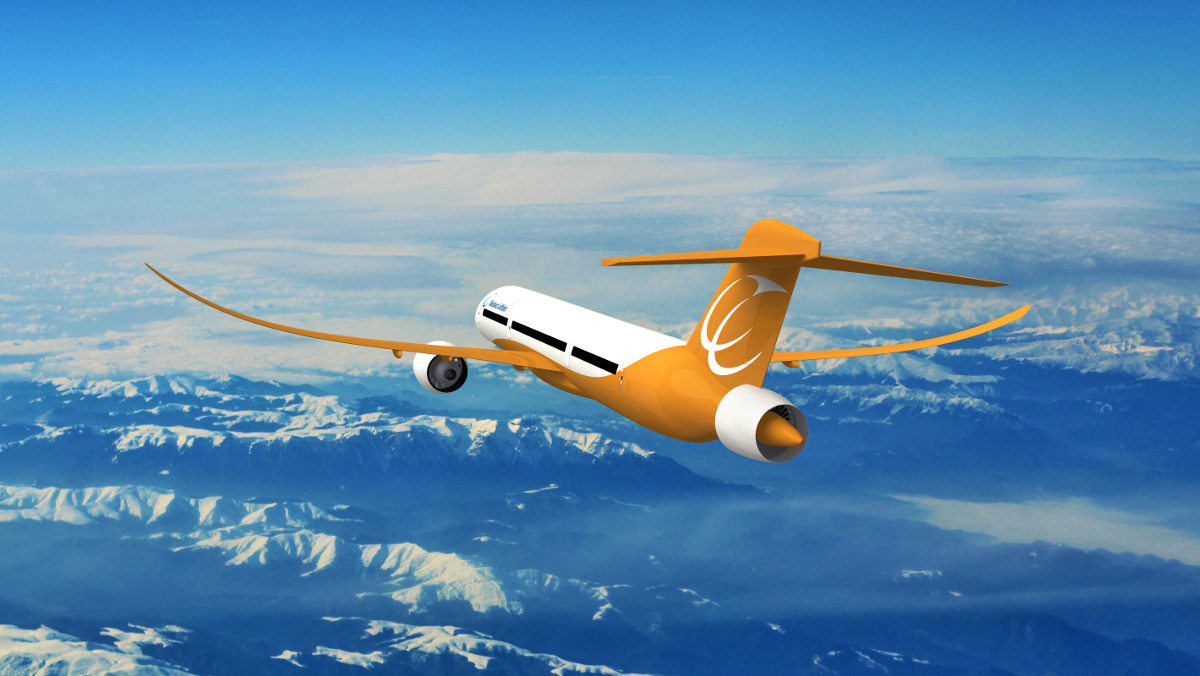
\includegraphics[keepaspectratio, width=0.6\textwidth]{images/chap1/centreline_concept.jpg}
	\caption{CENTRELINE concept, proposed by the CENTRELINE European consortium~\cite{bib:seitz_2018}.}
	\label{fig:centreline}
\end{figure}
Works on the CENTRELINE confirm the potential benefits coming from a propulsive fuselage with a BLI devices, already seen in the STARC-ABL. 
A major point of interest is the design of the powerplant, based on turboelectric configuration, and the technologies adopted~\cite{bib:bijewitz}. 

So far, two different potential technologies to be used in the hybrid and electric frame have been addressed: the DEP and the BLI, which seem to be the most promising features of such a kind of aircraft. 
Actually, these two aspects are not separated, but the DEP is synergistic with BLI, since each one enhances the effect of the other~\cite{bib:gohardani_book}. 
The main question is: which is the best geometry to be considered, to maximize the benefits coming from the DEP coupled with BLI? 
From the experience of the STARC-ABL, the BLI operates better when the reference length is higher: in configurations like the DRAGON one, its effects can be neglected because of the reduced chord length in the wing. 
This has been confirmed by another study on the Nautilius concept~\cite{bib:wiart}, and others~\cite{bib:arntz, bib:plas}. 

Possible candidate to answer the question is the Blended Wing-Body~\cite{bib:liebeck_1998}, in which the whole body is a lifting surface, and the reference length is large enough to take the maximum benefits from a possible integration with DEP and BLI~\cite{bib:bishara}. 
Besided this aspect, the BWB concept offers more space to locate distributed propulsion, maximizing the area subject to the combined effect of blowing and BLI. 
Last but not least, the BWB is a concept designed to maximise the aerodynamic, and thus it shows higher lift-to-drag ratio (values of 22-23 or above are foreseen): it has the potentiality to combine a morphological efficient architecture with enhancement benefits coming from the distributed propulsion. 

Hence, seen the very promising perspectives offered by the BWB, next section investigates more profoundly this configuration, to understand the basic aspects and problems, in order to prepare the field for the discussion regarding a possible integration with hybrid propulsion. 

\subsection{Blended Wing-Body aircraft}
\label{subsec:chap1_bwb}

On a classical TAW configuration, the fuselage is only aimed to carry passengers and luggages, but it is solely a source of drag, being a non lifting component. 
To generate lift in a more efficiency way, it would be better to have all the components generating lift: this is the idea behind the Blended Wing-Body (BWB) concept, where even the passengers' cabin is aerodynamically shaped to contribute to the total aircraft lift. 
McDonnell \& Douglas company was the first to think at the utilisation of BWB for civil transport~\cite{bib:liebeck_1998}, followed by Boeing who proposed a configuration for 450 passengers~\cite{bib:liebeck_2004}: these two examples represent a milestone in the development of this configuration, and they are both shown in Fig.~\ref{fig:bwb_concept_example}. 
\begin{figure}[h!]
	\centering
	\begin{subfigure}{0.4\textwidth}
		\centering
		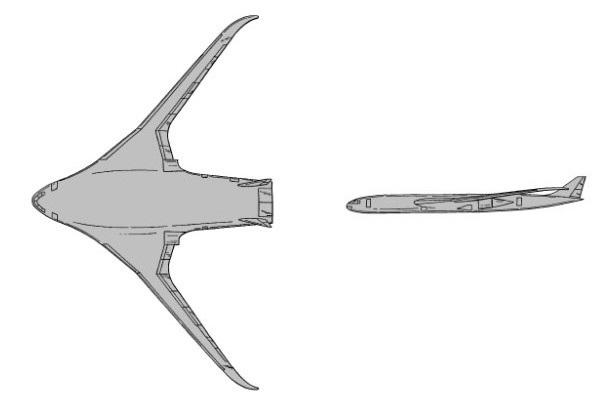
\includegraphics[keepaspectratio, width=\linewidth]{images/chap1/mcdonnell_bwb.jpg}
		\caption{BWB configuration, first proposed by McDonnell \& Douglas in 1998~\cite{bib:liebeck_1998}}
		\label{fig:mcdonnell_bwb}
	\end{subfigure}
	\hspace{10mm}
	\begin{subfigure}{0.4\textwidth}
		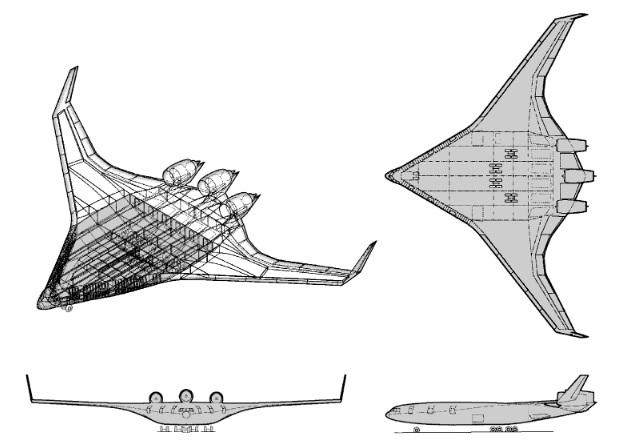
\includegraphics[keepaspectratio, width=\linewidth]{images/chap1/boeing_bwb.jpg}
		\caption{More advanced BWB concept, proposed by Boeing in 2004. This configuration is aimed to carry 450 passengers~\cite{bib:liebeck_2004}.}
		\label{fig:boeing_bwb_450}
	\end{subfigure}
	\caption{Main milestones in the Blended Wing-Body concept.}
	\label{fig:bwb_concept_example}
\end{figure}

The gain in the global lift-to-drag ratio comes mainly from the wetted area reduction: the integration of payload, lift, control surfaces and propulsion in an airfoil shaped centerbody helps to reduce the wetted area of about 30\%~\cite{bib:liebeck_1998}, resulting in a lower friction coefficient and a better efficiency. 
The maximum lift-to-drag ratio is estimated to be likely around 27~\cite{bib:torenbeek_bwb}.
Apart from the aerodynamics aspects, BWB shows also an improved structural efficiency, coming from the lower wing loading and large inertia relief~\cite{bib:liebeck_2004}.
Some studies also confirm that it has reduced the noise, relevant aspect close to ground, \textit{i.e.} during takeoff and landing~\cite{bib:bwb_n3_vol1}. 
Also, the BWB has more available volume to be used for the freight and the subsystem allocations, allowing more flexibility in the center of gravity positioning. 

Despite these advantages, several challenges arise in its design:
\begin{itemize}
	\item Since the cabin it is not cylindrical anymore, the pressurization generates a non-linear stress constraint which varies quadratically with the cabin's width (see Fig.~\ref{fig:pressure_constraint}), resulting in a more complex structural design~\cite{bib:liebeck_1998, bib:mukhopadhayay_2004, bib:mukhopadhayay_2005}. 
	Of course this leads to an increase in mass, compared to a conventional fuselage: the challenge is to design a shell to efficiently carry the pressurization loads, saving weight.
	\begin{figure}[h!]
		\centering
		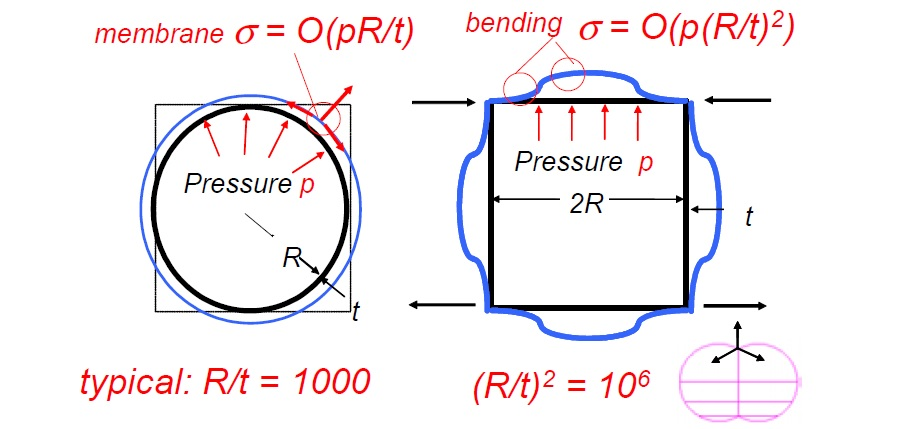
\includegraphics[keepaspectratio, width=0.6\textwidth]{images/chap1/pressurization_constraint.jpg}
		\caption{Different load distributions due to pressurization in a circular (left) and non-circular (right) cabin.}
		\label{fig:pressure_constraint}
	\end{figure}

	\item The BWB is a tailless configuration, so the airfoil design is a key point to obtain a longitudinally stable aircraft~\cite{bib:nickel}, otherwise fly-by-wire systems for the active control have to be inserted, with penalties in weight.
	
	\item Generally, the centerbody trailing edge is used to trim the aircraft at low speed: there is less place for high lift devices and thus $C_{L,\max}$ is reduced with respect to a conventional aircraft.
	
	\item Because of the airfoil-shaped centerbody, the landing gears positioning may represent an issue. 
	In order to have enough space available for this component, the relative thickness must be oversized, and this aspect is more critical especially for small BWB (short and medium range). 
\end{itemize}

These drawbacks make the interest in this concept being lost, because of the high commercial risk; however, it has emerged again in past years.
Nickol et al.~\cite{bib:nickol} considered the BWB as the most promising concept for the aviation environmental sustainability; in the N+3 project the BWB has been deeply studied to assess its performance: the final report from NASA represents a milestone because it provides a comprehensive study of different aspects~\cite{bib:bwb_n3_vol1}, together with an appendix with all the models~\cite{bib:bwb_n3_vol2}. 
Centracchio et al.~\cite{bib:centracchio} got almost the same results as Nickol, comparing a BWB concept with long range best-in-class aircraft.
TU Delft presented two works, one related to the cabin design~\cite{bib:vos_bwb}, and the second one about the parametrization and low fidelity models for evaluate the weights~\cite{bib:brown}; ONERA~\cite{bib:defoort} proposed an OAD procedure for its sizing within the CICAV project; AGILE project studies the definition of an OAD procedure for the BWB sizing, in their paradigma~\cite{bib:prakasha, bib:anisimov}, ISAE-Supaero, together with Airbus, mainly addressed with two Ph.D. projects the problem of the handling qualities~\cite{bib:saucez, bib:denieul}.
Also, it is to mention the study of Bonet, who analysed a scaled BWB geometry in wind tunnel~\cite{bib:bonet}, to confirm numerical results, and the X-48 demonstrator~\cite{bib:boeing_x48}, built from Boeing and NASA on the basis of Liebeck's work~\cite{bib:liebeck_2004} to study control within a flight test campaign, and the experimental work of Cranfield University for the VULCAN concept~\cite{bib:perry}.
Finally, DZYNE (a company based in California, USA) presented a new concept~\cite{bib:dzyne_bwb}, based on an innovative landing gear sizing, which opens this concept for small size, without the drawback of the oversized thickness-to-chord ratio.
They announced the construction of a BWB for an entry into service in the next decade, covering different segments, from the business to long range.
They called it ASCENT, and a visualisation of this concept is provided in Fig.~\ref{fig:dzyne_bwb}, taken from the work of Page et al.~\cite{bib:dzyne_bwb}.
\begin{figure}[h!]
	\centering
	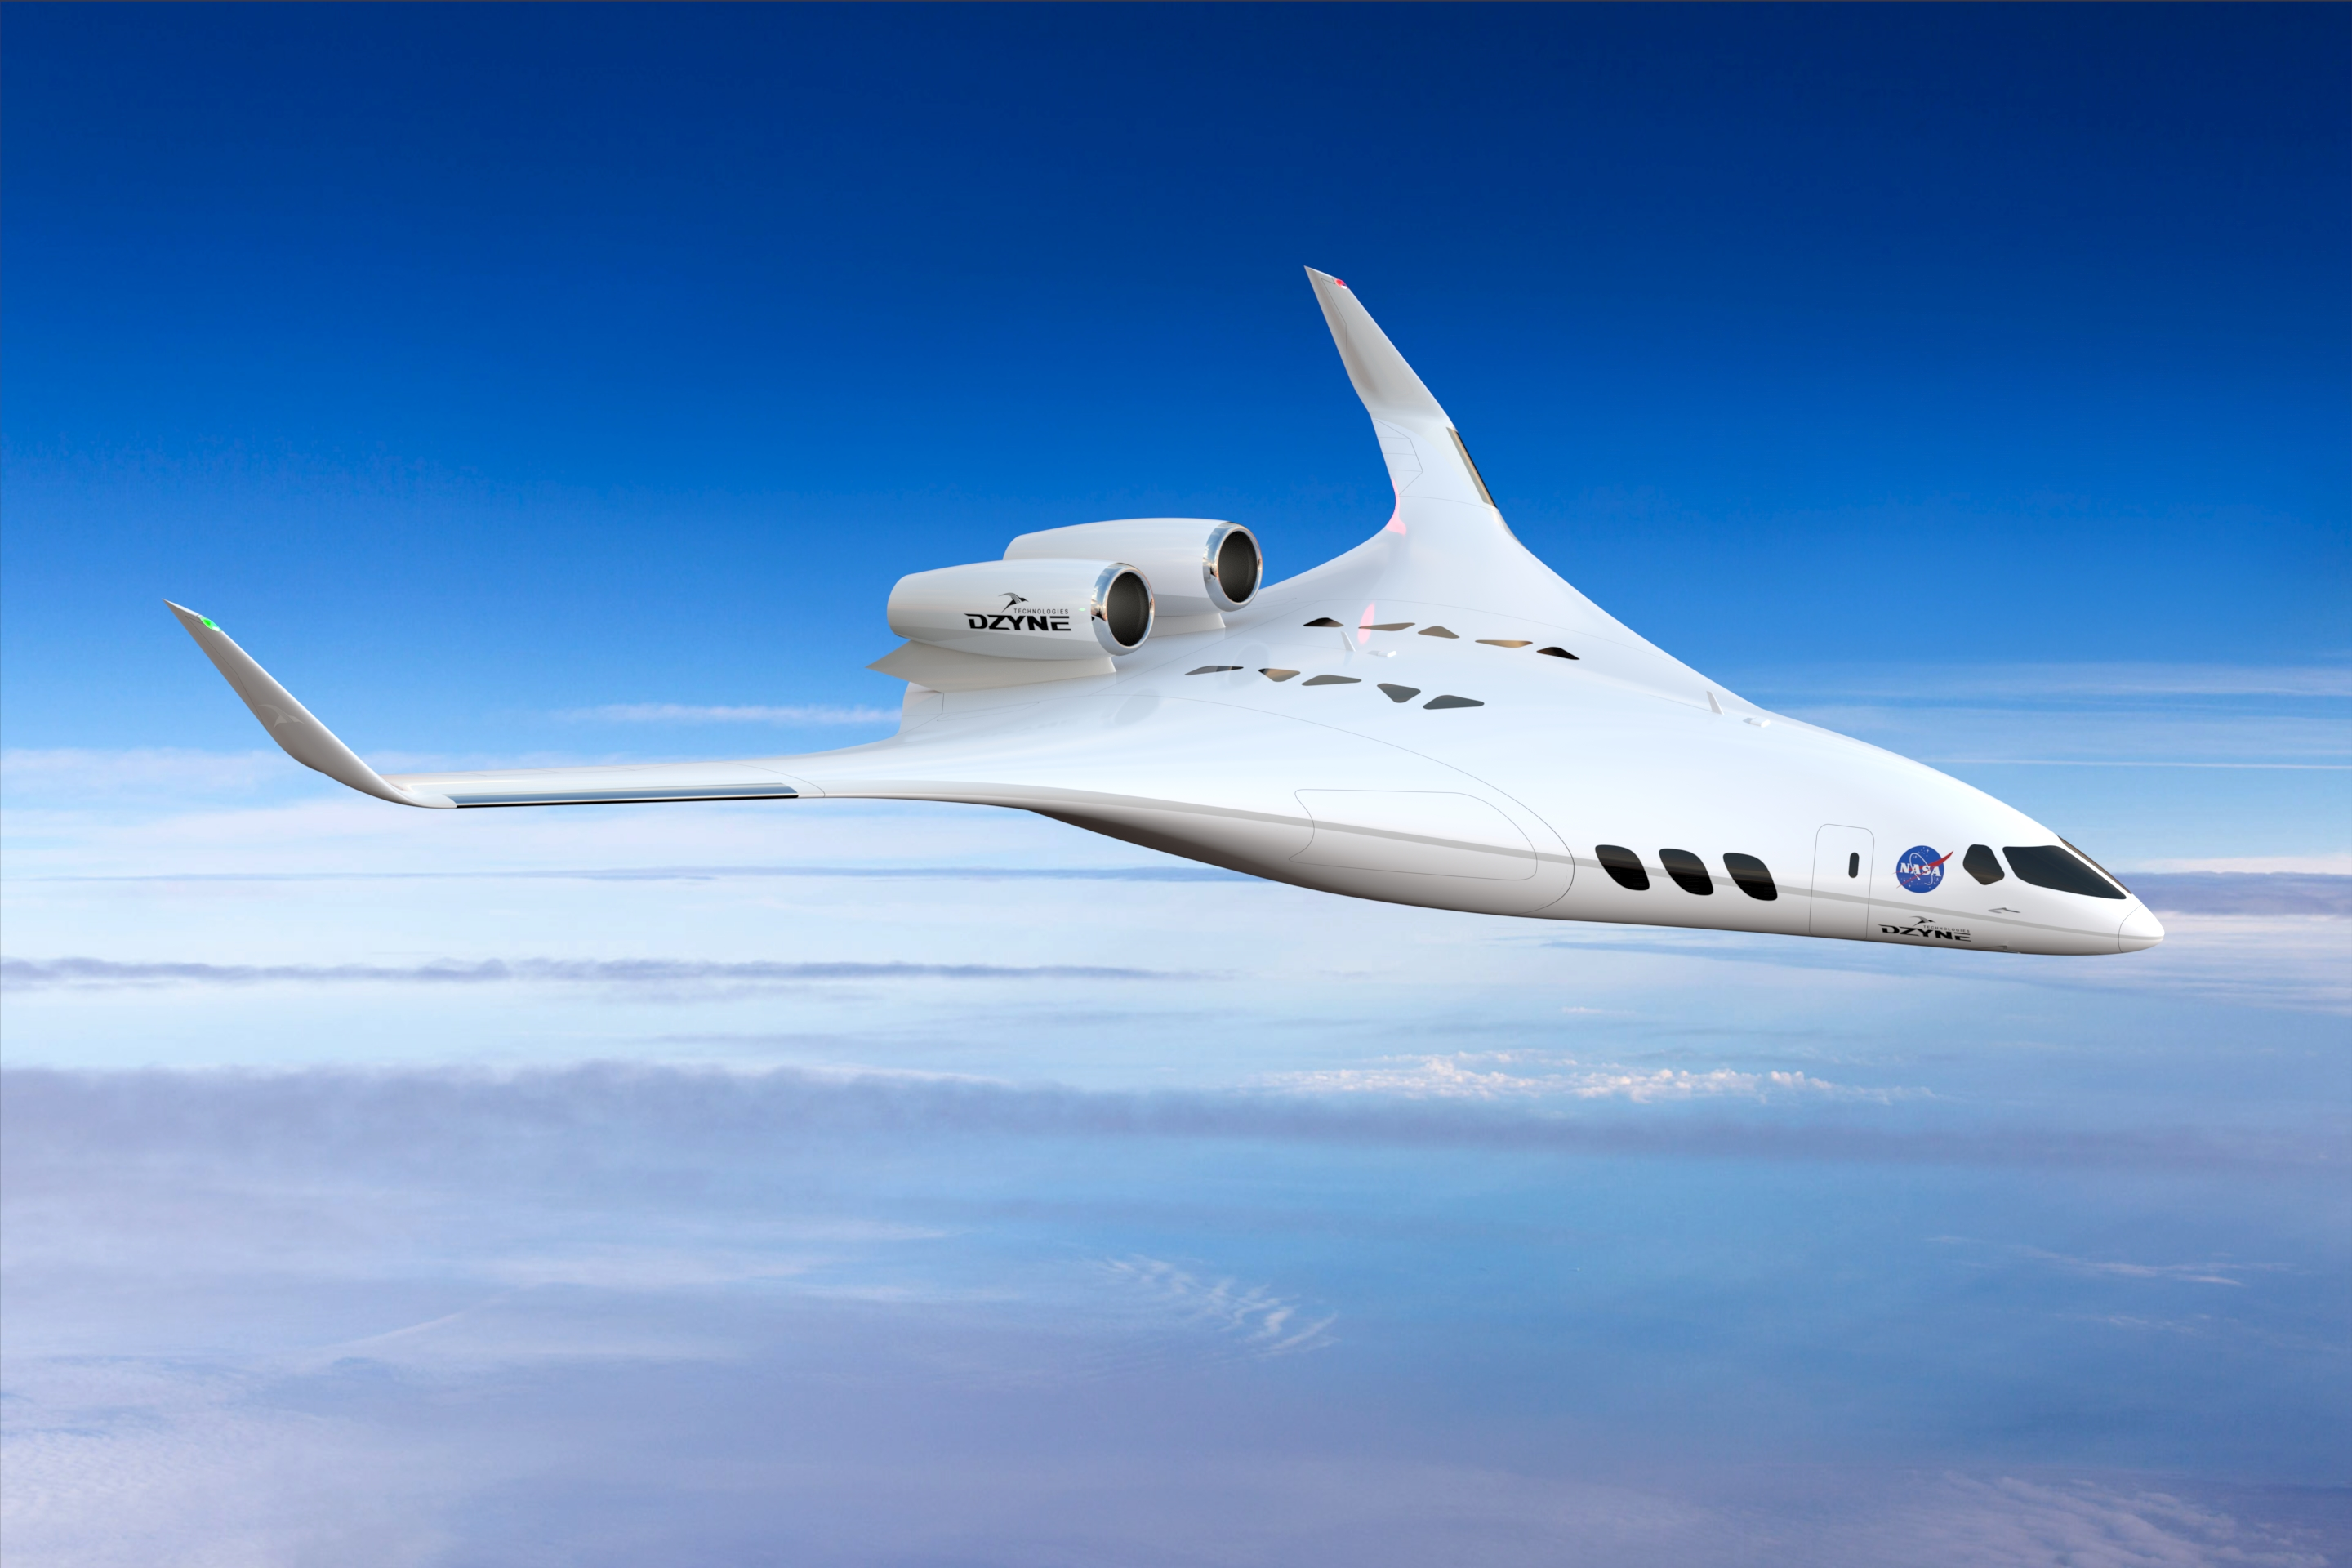
\includegraphics[keepaspectratio, width=0.5\linewidth]{images/chap1/dzyne_bwb.jpg}
	\caption{Rendering of the BWB Ascent 1000, announced by DZYNE and expected to fly in next years~\cite{bib:dzyne_bwb}.}
	\label{fig:dzyne_bwb}
\end{figure}

The examples above indicate how large is the interest in this concept; they are not exaustive of the whole literature on the topic.
Most of cited works cover only structural and aerodynamics aspects, using high fidelity; a minor part is instead deputed to handling qualities and control laws. 
At this stage there are only two evidences in literature of a revised sizing process for the BWB: NASA has implemented surrogate model for the cabin design, with aerodynamics correction, in its in-house code called FLOPS~\cite{bib:bradley_bwb}, but its development has been stopped~\cite{bib:brelje_biblio}.
Van Dommelen and Vos~\cite{bib:van_dommelen} presented a conceptual tool for the BWB design, based on classical methods that can be found in Roskam's books~\cite{bib:roskam_partI}. 

Another difficulty is that there is no availability of public reference data, to build surrogate models to use in preliminary design, with some exceptions as the FLOPS code, the aforementioned work of Van Dommelen and Vos~\cite{bib:van_dommelen}, and the database of NACA for the Northrop YB-49 aircraft, which is a delta wing aircraft, precursor of modern BWB~\cite{bib:robinson, bib:ashkenas}.
In the following two paragraphs, the problem of structural and aerodynamics design for a BWB is addressed, to prepare the field for a possible modelling approach, to be integrated in the conceptual design cycle.

\subsubsection{Structural design of Blended Wing-Body concept}
\label{subsubsec:chap1_bwb_structure}

The cabin structure is the most challenging aspect in designing the BWB: it must carry passengers (and eventually payload) and sustain both pressurization and aerodynamics loads. 
In literature it is possible to find three main propositions: integrated, segregated and oval structure. 
The first two were proposed by Liebeck~\cite{bib:liebeck_1998}, the third one has been explored by Vos et al.~\cite{bib:vos_bwb}. 
Vos et al. also suggest the following element to be considered when analyzing the cabin design:
\begin{itemize}
	\item Design simplicity; 
	\item Passenger evacuation;
	\item Passenger comfort;
	\item Structural efficiency; 
	\item Aerodynamics efficiency.
\end{itemize} 

The three cabin concepts have been considered by different authors dealing with structural design~\cite{bib:mukhopadhayay_2004, bib:mukhopadhayay_2005, bib:qian, bib:hansen}; more details about are reported in Appendix~\ref{app:bwb_cabin_design}. 
What is of interest in this context is the decision analysis reported in Table~\ref{tab:bwb_cabin_structure_synthesis} and based on the cited work.
In Table~\ref{tab:bwb_cabin_structure_synthesis}, a value of +1 is assigned whereas there is an advantage using a certain concept, 0 if an aspect may be an issue, but no relevant and -1 whereas a concept introduces a penalty. 
\begin{table}[!h]
	\centering
	\begin{tabular}{l| c| c| c|}
		\cline{2-4}
		& Integrated & Segregated & Oval \\
		\hline
		\multicolumn{1}{|l|}{Design complexity} & +1 & -1 & -1 \\
		\multicolumn{1}{|l|}{Passenger evacuation} & +1 & -1 & +1 \\
		\multicolumn{1}{|l|}{Passenger comfort} & 0 & +1 & +1 \\
		\multicolumn{1}{|l|}{Structural efficiency} & 0 & +1 & +1 \\
		\multicolumn{1}{|l|}{aerodynamics efficiency} & +1 & +1 & 0 \\ 
		\hline
	\end{tabular}
	\caption{Decision matrix for the three BWB cabin concepts proposed in literature. Values are assigned as follow: +1 if there is a good improvement, 0 if it may be an issue, but not relevant and -1 if it introduces a penalty.}
	\label{tab:bwb_cabin_structure_synthesis}
\end{table}

Table~\ref{tab:bwb_cabin_structure_synthesis} shows that the most interesting concept is the integrated one, since it conjugates a non complex design with acceptable passenger comfort and evacuation and good structural and aerodynamics efficiency: indeed, it has been largely used in different studies on the BWB structural design~\cite{bib:pitera, bib:kawai, bib:hileman_bwb, bib:bradley_bwb, bib:cheng}. 
These works use finite element method, with a detailed structure, to get an estimation of the structural mass of BWB: van Dommelen and Vos collected the available data from literature in their work~\cite{bib:van_dommelen}; Table~\ref{tab:bwb_struc_masses} sums up their review. 
\begin{table}
	\centering
	\begin{tabular}{l c c c}
		\hline
		\textbf{Aircraft} & \textbf{Ref.} & \textbf{Number of passengers} & \textbf{Structural mass [t]} \\
		\hline
		OREIO & \cite{bib:pitera} & 224 & 54.9 \\
		N2A & \cite{bib:kawai} & 262 & 51.6 \\
		SAX-40 & \cite{bib:hileman_bwb} & 215--236 & 47.6 \\
		BWB-250 & \cite{bib:bradley_bwb} & 250 & 38.3 \\
		BWB-450 & \cite{bib:bradley_bwb} & 450 & 68.9 \\
		\hline
	\end{tabular}
	\caption{Structural masses for different BWB concepts available in literature. Adapted from~\cite{bib:van_dommelen}.}
	\label{tab:bwb_struc_masses}
\end{table}
It is to note that no less than 215 passengers are considered. 
In general, the more complex structure introduces a penalty in weight: for comparison, the structural mass of the Airbus A321, designed for 236 passengers, is 48.5~\si{\tonne}, which is lighter than the data of Table~\ref{tab:bwb_struc_masses}, except for the BWB-250 which uses very aggressive hypothesis for the material. 
However, this comparison is only indicative, since a lot of information about the detailed design adopted are missing, but it gives in any case an idea about the expected order of magnitude. 

Bradley was the only one to try to get a surrogate model, for an easy application in preliminary design phase~\cite{bib:bradley_bwb}.
In his work, he considered different BWB configurations, varying from 200 to 450 passengers, all of them shown in Fig.~\ref{fig:bwb_bradley_concept}. 
\begin{figure}[h!]
	\centering
	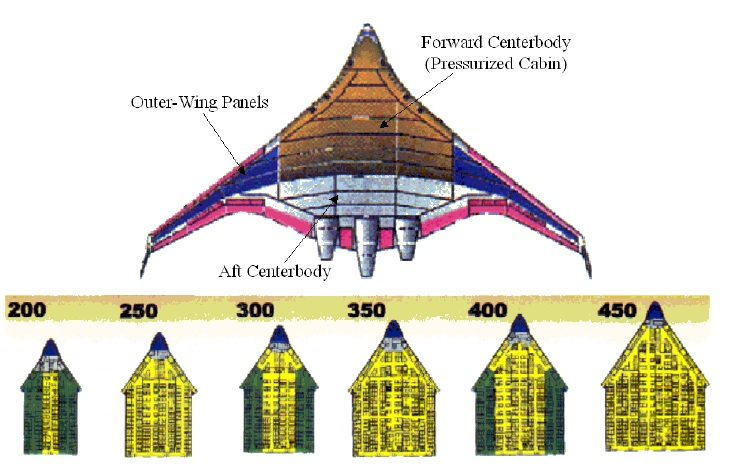
\includegraphics[keepaspectratio, width=0.6\textwidth]{images/chap1/bwb_bradley_concept.jpg}
	\caption{Blended Wing-Body cabin design, according to Bradley~\cite{bib:bradley_bwb}}
	\label{fig:bwb_bradley_concept}
\end{figure}
The concept for the cabin is the integrated one: he assumed that the cabin is divided into bays by the ribs, and each bay can allocate a single aisle with two column of passengers.
Then, he built the models and ran FEM analyses, for different configurations, to estimate the cabin mass. 
With the data obtained, he aimed to find a surrogate model, where the cabin mass formula takes the following shape:
\begin{equation}
	\label{eq:cabin_mass_general}
	m_{cabin} = a\left(m_{TO}\right)^b\left(S_{cabin}\right)^c
\end{equation}
where $m_{cabin}$ is the mass of the cabin, $m_{TO}$ the maximum takeoff weight, $S_{cabin}$ the cabin surface and $a$, $b$, $c$ some constants to be determined. 

Using the regression analysis, the three constants may be determined, finally having
\begin{equation}
	\label{eq:bwb_cabin_mass}
	m_{cabin} = k_s 0.316422 \left(m_{TO}\right)^{0.166552}\left(S_{cabin}\right)^{1.061158}
\end{equation}
where $k_s$ is a scaling factor to consider different technologies, that in his work was calibrated on the Boeing data, resulting to be $k_s=5.698865$. 
This model has then been implemented into FLOPS, a NASA in-house code for the preliminary design, to size a BWB, but as already said it has been abandoned and no further development came out. 

The main limiting factor of the model proposed by Bradley is that it uses very aggressive hypothesis on the composite material, and it considers also one load case, with reference values from Liebeck~\cite{bib:liebeck_2004}; also, it does not consider the effect of the cabin thickness. 
Despite these drawbacks, it has been successfully applied in other projects~\cite{bib:liu} and still remains a good starting point for further development of a conceptual tool for the BWB.

Some authors carried out also a dynamic structural analysis for the BWB, in order to capture the vibration modes~\cite{bib:yingsong, bib:weihua, bib:stroscher, bib:carlsson}.
Despite the research on this field is very limited, results show that a BWB configuration suffers less of flutter problem, due to stiffer structure, but torsional and bending moment are more critical. 
The most complete work is the one presented by Stettner and Voss~\cite{bib:stettner}, who included also handling qualities together with aeroelasticity analysis, showing that the trim problem is not trivial. 
Their main conclusion is that the BWB configuration needs more control surfaces than conventional aircraft to ensure stability and controllability, especially at low speed condition, where the bending and torsional moments are more relevant. 

\subsubsection{Aerodynamics tradeoff for the Blended Wing-Body}
\label{subsubsec:chap1_bwb_aero}

The BWB design is mainly done for improving aerodynamics performances, achieved by having a single lifting body and a reduced wetted area~\cite{bib:liebeck_1998}. 
The airfoil design is then a priority for the aerodynamics design, in particular for the cabin section, in which the thickness has to be large enough to allocate the passengers. 

The BWB design is highly influenced by equilibrium and stability constraints: for longitudinal equilibrium, the center of gravity should be afterwards the aerodynamics center~\cite{bib:anderson_perfo}, but this positioning implies statically unstable aircraft.
Herein, classical notation for aircraft stability is considered: momentum is positive when it is clockwise~\cite{bib:roskam_perfo, bib:roskam_flight_dynamics}. 
In conventional aircraft an horizontal tail is designed to make the aircraft stable, but being the BWB a tailless concept, there are no elements for trim. 
The goal is to have a small positive momentum coefficient around the center of gravity $C_{M_{cg}}$, at limit zero, which represents the best condition. 
Most of the airfoils, instead, are designed to obtain a negative $C_m$~\cite{bib:abbott}, the only exception is represented by the reflex airfoil. 
These types of airfoils have a trailing edge camber line lifter upward, generating a positive $C_m$, and this effect makes them perfect for the BWB design~\cite{bib:alex, bib:wang}.
The most common reflex airfoil family is represented by the NACA 5-digit series~\cite{bib:abbott}, but other families have been developed, like the MH family, deputed for the use on tailless aircraft~\cite{bib:mh_airfoiltool, bib:eppler}. 

However, using a reflex airfoil could compromise the transonic behaviour~\cite{bib:sargeant}: due to three-dimensionality, most of the centerbody lift is generated at the front.
For a reflex airfoil, this zone needs more curvature to counteract the loose of lift in the afterward part. 
As such, the critical and drag divergence Mach numbers are lower than that of a conventional airfoil, with potentially issue in the transonic regime. 
To limit the contribution to compressibility, as general rule, the thickness-to-chord ratio for the centerbody must not exceed 18\%~\cite{bib:kozek, bib:ikeda}.

The path just described helps the section design, but on a global point of view the aerodynamics load and the target $C_l$ distribution drive the design~\cite{bib:anderson_perfo}. 
It is to recall that the aerodynamics load is a punctual quantity, associated to the lift distribution as follow
\begin{equation}
	\label{eq:aero_load}
	\gamma\left(\eta\right) = \frac{c\left(\eta\right)C_l\left(\eta\right)}{2b}
\end{equation}
where $\eta=\frac{y}{\frac{b}{2}}$ is the non dimensional coordinate in the spanwise direction, $c$ and $C_l$ the local chord and lift coefficient, and $b$ the wing span. 
Integrating this quantity over the span the global $C_L$ is obtained
\begin{equation}
	\label{eq:global_cl_aero_load}
	C_L=AR\int_{0}^{\frac{b}{2}}\gamma\left(\eta\right)d\eta
\end{equation}
with $AR$ being the aspect ratio. 

On a conventional aircraft, with an aspect ratio above 5-6, the Prandtl theory gives results with a good accuracy; the reduced aspect ratio of the BWB, however, suggests that the Prandtl theory is not valid anymore, but the Jones theory may be more indicated~\cite{bib:cdn_notes}. 
This theory states that, in case of a low and untwisted aspect ratio wing, the aerodynamics load follows the elliptical distribution, and then from one hand the induced drag is minimised, but from the other hand it shows high $C_l$ at the wing tip for untwisted configuration, with consequently issues for the transonic performance and controllability because of the impossibility to use ailerons. 
Qin et al.~\cite{bib:qin} studied the load distribution on a BWB configuration, using RANS methods, and confirmed that the elliptical distribution is obtained with an untwisted wing. 
To balance the induced drag and the transonic performance, they added a twist distribution, using the inverse design technique, and found that the best load is obtained averaging and elliptical load with a triangular one. 
The inverse design is done using a low fidelity method (panel method); the results are then assessed on a set of points with high fidelity (RANS method).
Their results are presented in Fig.~\ref{fig:qin_cl_target} and Fig.~\ref{fig:qin_load_target}, as well as in Table~\ref{tab:qin_load_results}. 
With the average load, the lift coefficient at the tip is not as high as the elliptical case, avoiding stall and compressibility problems, but it is not as low as the triangular distribution, avoiding to increase the angle of attack to find the right lift. The elliptical-triangular distribution has a lower global $C_L$, but the difference is small (around 2\%); from Table~\ref{tab:qin_load_results} it can also be noted that, even if for an elliptical distribution the induced drag is lower, the wave drag is instead higher and in the end the global $C_D$ is higher, confirming that it is not the global optimal distribution, but only with respect to the induced drag. 
\begin{figure}[!h]
	\centering
	\begin{subfigure}{0.5\textwidth}
		\centering
		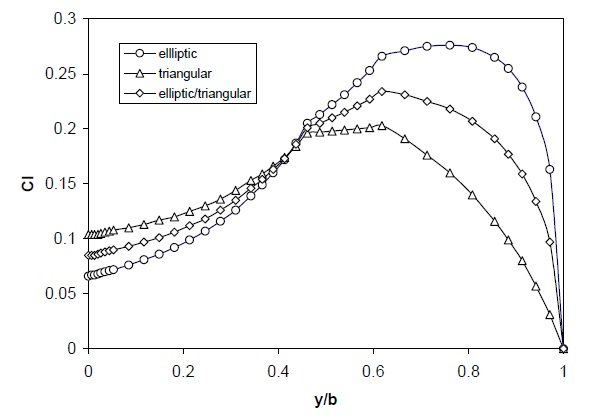
\includegraphics[keepaspectratio, width=\linewidth]{images/chap1/cl_target.jpg}
		\caption{Target lift distribution as a function of non dimensional span, for the case examinated by Qin et al.~\cite{bib:qin}.}
		\label{fig:qin_cl_target}
	\end{subfigure}
	\begin{subfigure}{0.5\textwidth}
		\centering
		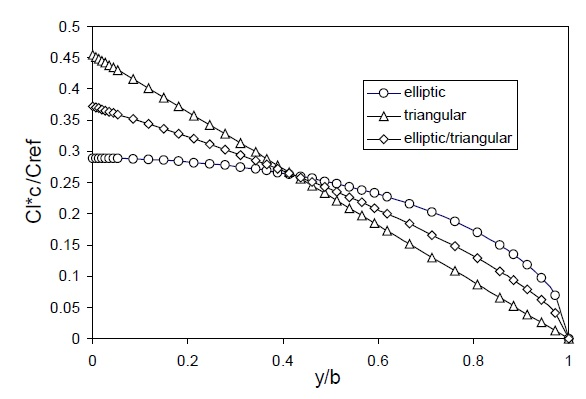
\includegraphics[keepaspectratio, width=\linewidth]{images/chap1/load_target.jpg}
		\caption{Target aerodynamics load distribution as a function of non dimensional span, for the case examinated by Qin et al.~\cite{bib:qin}.}
		\label{fig:qin_load_target}
	\end{subfigure}
	\caption{Aerodynamics tradeoff for a BWB, from the work of Qin et al.~\cite{bib:qin}.}
	\label{fig:qin_results}
\end{figure}

\begin{table}[!h]
	\centering
	\caption{Comparison of performance for the different target distributions examinated in the work of Qin et al.~\cite{bib:qin}, related to a BWB configuration.}
	\begin{tabular}{l l l l l l}
		\hline
		{Twist distribution}  & {$C_L$} & {$C_{D}$} & {$C_{D_{i}}$} & {$C_{D_{f}}$} & {$C_{D_{w}}$} \\
		\hline
		Baseline     & 0.4136 & 0.03268 & 0.02504 & 0.00764 & 0.00407 \\
		Elliptic     & 0.4102 & 0.02837 & 0.02031 & 0.00806 & 0.00209 \\
		Averaged     & 0.4090 & 0.02783 & 0.02008 & 0.00774 & 0.00180 \\
		Triangular   & 0.4071 & 0.02866 & 0.02083 & 0.00783 & 0.00161 \\
		\hline
	\end{tabular}
	\label{tab:qin_load_results}
\end{table} 

The work just described is interesting for two main reasons: it confirms that the Jones theory can be applied on a BWB, and it is the first evidence of a strategy in which the low fidelity is used to design a BWB, with the results being lately assessed using high fidelity. 
For what has been extensively said in Section~\ref{sec:chap1_ac_design_cycle}, at conceptual design is a key point to have fast and reliable methods, and Qin suggested a first path to follow in the conceptual aerodynamics design of the BWB. 

Beside this work, the other major references about the BWB aerodynamics used RANS method for the design: the design point is chosen, based on the target $C_L$, and then the configuration is resized until it matches the requirement.
This approach has the drawback that there are no information about the other operating points at which the BWB flies~\cite{bib:li_bwb}.
 
In the past year, fostered in the progress made in the MDO techniques~\cite{bib:martins_mdo}, different authors used optimisation algorithm for the geometry design, included the airfoil.
The first ones were Mader and Martins~\cite{bib:mader}, who tested on a flying wing this approach. 
Later Lyu and Martins set up an optimisation routine for a BWB, based again on a RANS solver~\cite{bib:lyu}. 
They defined a total of 273 design variables, regarding the twist distribution, the airfoil shape, the local sweep and chord, and the span, as shown in Fig.~\ref{fig:lyu_bwb_dv}. 
They investigated the impact of the various constraints and design variables on optimised BWB: trim and static stability were investigated both for the design and off design conditions. As a result, it was possible to find the best combination of wing twist and airfoil reflex to maximize the efficiency, satisfying at the same time trim and stability constraints.
\begin{figure}[h!]
	\centering
	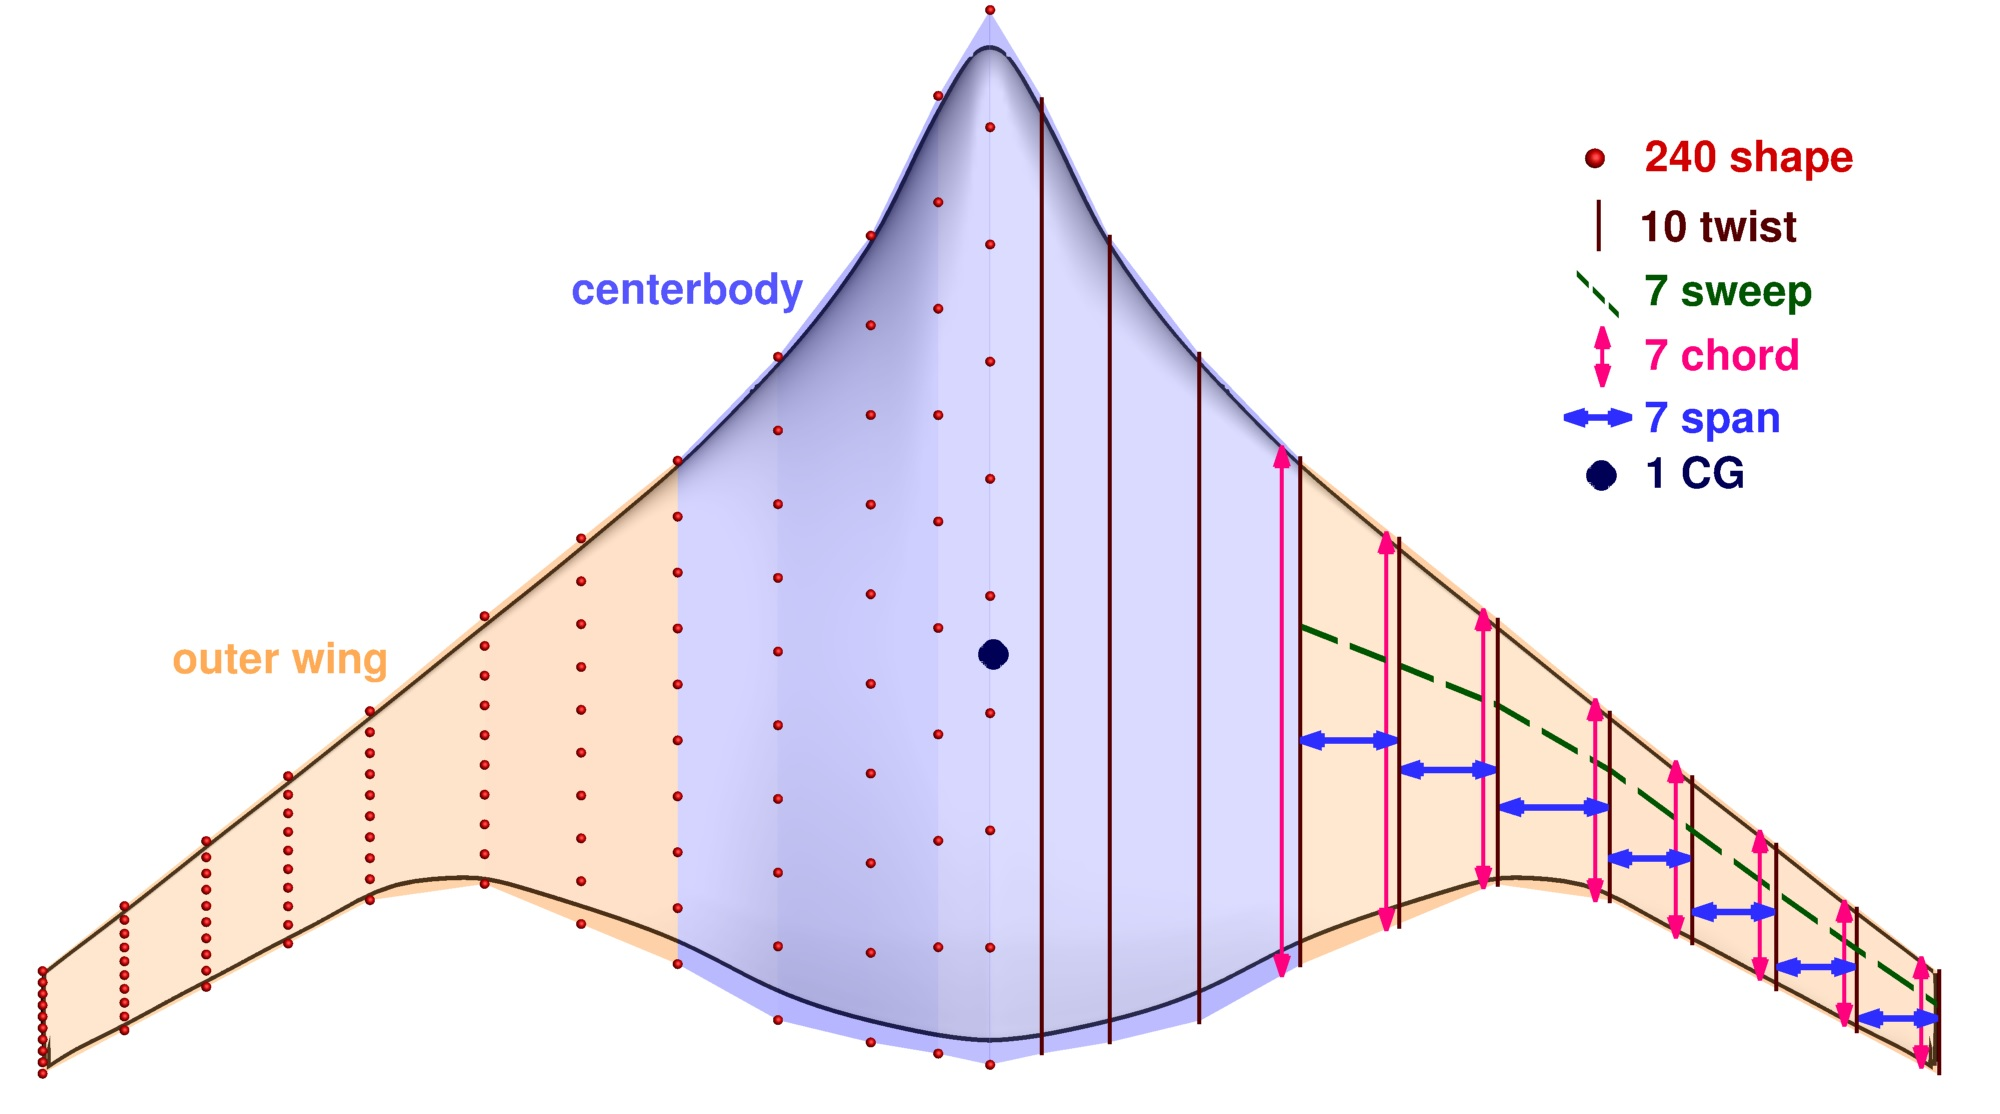
\includegraphics[keepaspectratio, width=0.8\textwidth]{images/chap1/bwb_martins_design.jpg}
	\caption{Shape and planform design variables considered in the work of Lyu and Martins, for the BWB optimisation~\cite{bib:lyu}. }
	\label{fig:lyu_bwb_dv}
\end{figure}

Liou et al.~\cite{bib:liou_2016, bib:liou_2017} carried out a similar work, including also the engine integration within the airframe, on a NASA hybrid configuration. 
Through all these works, that do not cover all the bibliography for the subject, the RANS-based aerodynamics shape optimisation method has been well assessed: they demonstrated that is a pratical tool for the BWB aerodynamics design. 
The main drawback is the computational cost: it is unfeasible to carry out such simulations on a single processor, and then a multiprocessor architecture is needed; still, the computational cost remains high. 
As example, in the work of Lyu and Martins~\cite{bib:lyu}, a single optimisation converged in 10~\si{\hour} using 240 processors. 
Thus, it is unfeasible to integrate CFD analysis for aerodynamics within the conceptual design loop, but it can be used to validate low fidelity methods or to define surrogate models, based on few set of geometrical parameters. 

On this direction, a first step has been done by Prince et al.~\cite{bib:prince}, who tested a commercial code, based on panel method, and compared the results with a RANS solver: they reports a maximum error of 10\% for the BWB configuration, which may be acceptable at conceptual design. 
Also, the maximum difference occurs at very high Mach number, when the compressibility effects are dominating the flow field; at low Mach numbers the agreement between the methods is much more marked. 

This work and the already mentioned work of Qin et al. represent the two most interesting cases in which theory or low fidelity methods are applied for the BWB configuration; further investigation is needed to get more reliable results, or even surrogate models to replace the empirical equations suggested by Roskam and extensively used for conventional aircraft~\cite{bib:roskam_partVI}.

The overview on the BWB concept ends up here: the next paragraph will discuss the possible integration among the innovative technologies identified to finally converge towards a potential solution capable to match environmental goals. 

\section{The research problem} 
\label{sec:chap1_research_problem}

\subsection{Towards a promising solution for aviation sustainabilityn}
\label{subsec:chap1_conf_proposition}

The previous section reports a review of the most promising innovative technologies considered in literature, to match the aviation's environmental goal for the upcoming years. 
Among all the possibilities, the hybrid and electric propulsion has been taken into account: from the studies reported came out that this technology has been identified as the best choice for the next generation aircraft. 
In particular, the main feature is that it opens new and still unexplored possibilities, \textit{e.g.} the integration with a BLI device to improve aerodynamics. 
Distributed propulsion is identified as a solution to take advantage of the hybrid propulsion, especially because DEP enhances the benefits coming from the BLI, and viceversa. 

Then, the focus has been shifted on the best architecture for this integration: in fact, BLI to be efficient requires large chords, otherwise its impact is negligeable. 
The solution is the Blended Wing-Body architecture, which is characterised by the integration of aerodynamic, structure and payload. 
By definition, the BWB is a whole lifting surface, and offers very large chords. 
So, it comes almost naturally to consider the Blended Wing-Body featuring distributed electric propulsion as possible solution for next generation aircraft. 
In fact, it takes advantages from all the innovative aspects described above. 
It is to note that innovation is brought on a two different level: propulsive, with the introduction of a new power plant, and structural, with a disruptive concept mainly designed for high aerodynamics performances. 

The intuition of BWB with DEP is confirmed by one of the most known concept proposed by NASA, within the N+3 program: the N3-X turboelectric concept~\cite{bib:kim_n3x_2008}. 
This concept, shown in Fig.~\ref{fig:nasa_n3x}, has been designed to be competitor of the Boeing 777 in terms of range and payload, and it is characterised by the integration of a distributed electric propulsive system within the BWB architecture. 
The entry into service goal is set to 2040: technological assumptions are made in perspectives for this horizon. 
\begin{figure}[!h]
	\centering
	\includegraphics[keepaspectratio, width=0.6\textwidth]{images/chap1/nasa_n3x.jpg}
	\caption{NASA N3-X concept~\cite{bib:kim_n3x_2008}.}
	\label{fig:nasa_n3x}
\end{figure}
The propulsors are mounted at the trailing edge, with the electric power coming from two generators, located at the wing tip; studies from Kim et al.~\cite{bib:kim_2013} show that this configuration enables very high propulsive efficiency, thanks to the partial electrification of the engine's cycle. 
The N3-X has been presented for the first time in 2008: both Kim~\cite{bib:kim_n3x_2008} and Felder~\cite{bib:felder_2009} performed preliminary studies to have a first estimation of its performance. 
Both the works showed that N3-X offers very good performance in terms of fuel reduction; as a consequence, deeper studies were conducted to confirm the preliminary results~\cite{bib:felder_2012, bib:kim_n3x_2014}, with refined trade-off for the weights~\cite{bib:brown_n3x}, noise and emission~\cite{bib:berton}. 
It has been estimated that the concept requires an amount of power in the order of 50~\si{\mega\watt}: such demand makes the superconducting technology and the associated cryogenic subsystems the only possible way to satisfy the requirements. 
In different works Rolls-Royce and the University of Strathclyde in UK collaborated on electrical system trades~\cite{bib:armstrong_n3x_2012, bib:armstrong_n3x, bib:armstrong} and the system safety analysis of such a complex architecture~\cite{bib:ross, bib:shaw_2014, bib:shaw_2015}. The assessment of performance shows a reduction of 70\% in fuel burn, compared to the Boeing 777~\cite{bib:felder_2011}, due to the partial electrification and the improved airframe; economic viability is demonstrated too~\cite{bib:goldberg}. 
The main issue with this concept is that it uses a very aggressive technology, and thus it introduces a large amount of technological risk for an EIS2040: Jansen et al.~\cite{bib:jansen} studied, for this case, the required individual technology for the electric subsystems, and they are really challenging even dealing with such a large technological horizon. 
Despite that, the N3-X is still a milestone for the integration of the hybrid propulsion within BWB airframe and the benchmarking for the fuel burn, noise and emission reduction. 

Beside the N3-X, other authors found an interest in the BWB featuring hybrid propulsion: Rodriguez presented the benefits coming from the BLI on a reference Boeing geometry~\cite{bib:rodriguez}, meanwhile Kok~\cite{bib:kok} and Campbell~\cite{bib:campbell_bli} separately studied the effects of combining DEP and BLI on a BWB configuration.
Finally, Ko et al.~\cite{bib:ko_bwb} set up a multidisciplinary optimisation formulation to get the optimal geometry with respect to the propulsive benefits. 
All these works report an improvement in the fuel efficiency above the 20-30\%.

So far, the N3-X is the most complete concept, but it has been studied considering individual disciplines, with specific high fidelity tools, but no OAD process is defined. 
Also, it is competitor of the Boeing 777, so it is designed for long range and 450 passengers, whereas the single aisle aircraft, as \textit{i.e.} the Airbus A320, represents the critical segment for emission (see Fig.~\ref{fig:aviation_emission_breakdown}), and in Boeing perspective it will be the segment with the major growing ratio~\cite{bib:boeing_outlook_market}. 

\subsection{Problem statement and proposed solutions}
\label{subsec:chap1_prob_statement}

This research, finally, has the objective to define an OAD process, at conceptual level, for the study of a BWB featuring DEP, in the same segment as the Airbus A320 (short/medium range, 150 passengers). 
An EIS 2035 is considered; to limit the risk associated to the concept, only non-cryogenic technology is considered. 
In fact, there is a lot of uncertainty about the cryogenic technology and its application for aviation on short term. 

The research problem can be summed up in the following question: 
\begin{mdframed}[hidealllines=true,backgroundcolor=green!20]
	\textbf{Research problem.} How will the conceptual design process can be revised for the study of an unconventional configuration that features an innovative hybrid powerplant?
\end{mdframed}
The answer is not obvious: conceptual design methods, described in Sec.~\ref{sec:chap1_ac_design_cycle}, are well assessed for a TAW aircraft configuration, but are not valid anymore for hybrid aircraft. 
The example of the N3-X, as well as the X-57, the STARC-ABL and others presented in Sec.~\ref{sec:chap1_key_innovative_techno}, show hybrid/electric aircraft have more interaction between disciplines than a conventional aircraft. 
As already remarked, even the Breguet equation does not hold yet and must be revised~\cite{bib:hepperle, bib:marwa}. 
The most representative case of the existing coupling is provided by aerodynamics and propulsion, that cannot be considered as separated disciplines, since each one impacts the other one. 
Pornet et al.~\cite{bib:pornet, bib:pornet_2014} presented a preliminary sizing procedure for hybrid aircraft, and they stressed in different points that integration of a new hybrid powerplant has an impact on all disciplines.
At that stage several assumptions have been done, that limit the application.  
Cinar et al.~\cite{bib:cinar_sizing} arrived at same conclusion; De Vries et al.~\cite{bib:devries_2018} presented instead a revised procedure for the sizing that includes aero-propulsive interaction, demonstrating on a test case of regional aircraft that the two disciplines cannot be considered separated anymore. 

More complications come considering the thermal management, which has been neglected in the three works cited above~\Cite{bib:pornet, bib:cinar_sizing, bib:devries_2018}: Freeman~\cite{bib:freeman} and Campbell~\cite{bib:campbell_prop} noted that thermal aspects cannot be neglected when considering electric architecture. 
Due to the large demand of power, dissipation due to Joule effect is significant, and cooling systems must be included to avoid problems related to structure's heating. 

A key point, addressed by Brelje and Martins, is that the classical design procedure relies on MDA, and its capability to deal with the problem of unconventional configurations is limited~\cite{bib:brelje_biblio}.
Research must focus more on a revised sizing procedure, based on Multidisciplinary Design optimisation (MDO)~\cite{bib:martins_mdo}; sometimes the notation MDAO (Multidisciplinary Design Analysis and Optimisation) is used to highlight the multidisciplinarity characterization. 
The MDAO, as defined by Martins and Lambe~\cite{bib:martins_mdo}, is a ``field of engineering that focuses on the use of numerical optimization for the design of systems that involve a number of disciplines and subsystems''.
MDO origins can be traced back to '60 years, when Haftka~\cite{bib:haftka_1973, bib:haftka_1975, bib:haftka_1977, bib:haftka_1979} and Schmit~\cite{bib:schmit_1960, bib:schmit_1965, bib:schmit_1981, bib:schmit_1984} started to extend their experience in the structural optimisation to other disciplines. 
In recent years, thanks to the improvements in computational science and the new resources available, MDO is become a powerful tool for aircraft design~\cite{bib:kroo, bib:manning, bib:antoine, bib:henderson, bib:alonso} and other engineering problems~\cite{bib:martins_mdo}. 
Moreover, it is recognised as the only solution to deal with the problem of unconventional configurations~\cite{bib:lyu, bib:raymer, bib:brelje_biblio}. 
Brelje and Martins demonstrated their assumption on another work~\cite{bib:brelje_model}, whereas they present a MDO tool for the optimisation of small electric aircraft. 
Despite the limiting assumptions in models used, they concluded that performances were indeed improved compared to a conventional MDA procedure. 
Also, they identified the problem of a full MDO formulation for aircraft design problem as still an open issue in literature. 

Finally, the answer to the research problem comes out. 
It can be divided into three subpoints, as follow: 
\begin{mdframed}[hidealllines=true,backgroundcolor=green!20]
	\textbf{Answer to research problem.} 
	The problem of sizing unconventional configurations with hybrid architecture for the thrust generation at conceptual level can be tackled through:
	\begin{itemize}
		\item The definition of new models, to consider the impact of the innovative architecture on geometry, structure, aerodynamics and performance evaluation;
		
		\item The application of a multifidelity approach, to calibrate the conceptual design methods with more refined simulations;
		
		\item The definition of a sizing procedure based on Multidisciplinary Design Analysis and Optimisation, because of its capability to establish tradeoff taking into account all the interactions between disciplines, particularly relevant for unconventional aircraft. 
	\end{itemize} 
\end{mdframed}

The definition of a MDAO formulation opens two related issues: ``Which are the models to use for the discipline, to account for innovative configurations?'' and ``Which is the best MDO formulation for aircraft design problem?''.
All these issues will be addressed in the manuscript; the two main Ph.D. objectives can be summed up considering these points: 
\begin{itemize}
	
	\item Set up of a complete multidisciplinary design analysis process for the sizing of the innovative concept and its performance evaluation;
	
	\item Choice of the most suitable multidisciplinary design optimisation formulation, in order to carry out an optimisation loop.
\end{itemize} 

It has been noted several times, and recalled here, that the test case of BWB with DEP presents two main innovations, one related to the propulsive architecture and another one to the overall configuration. 
To facilitate the development of a sizing procedure, the work is divided into three minor steps:
\begin{itemize}
	\item Study of a TAW configuration featuring distributed electric propulsion,
	\item Study of a medium range BWB, with conventional engines,
	\item Merge of the two previous concepts, to finally arrive at the BWB with distributed electric propulsion.
\end{itemize}

The Ph.D. roadmap, that shows this division into intermediate steps, is shown in Fig.~\ref{fig:phd_roadmap}.
This way to proceed allows also to study the two innovative aspects introduced separately, assessing their benefits in terms of aircraft performance individually. 
\begin{figure}[!h]
	\centering
	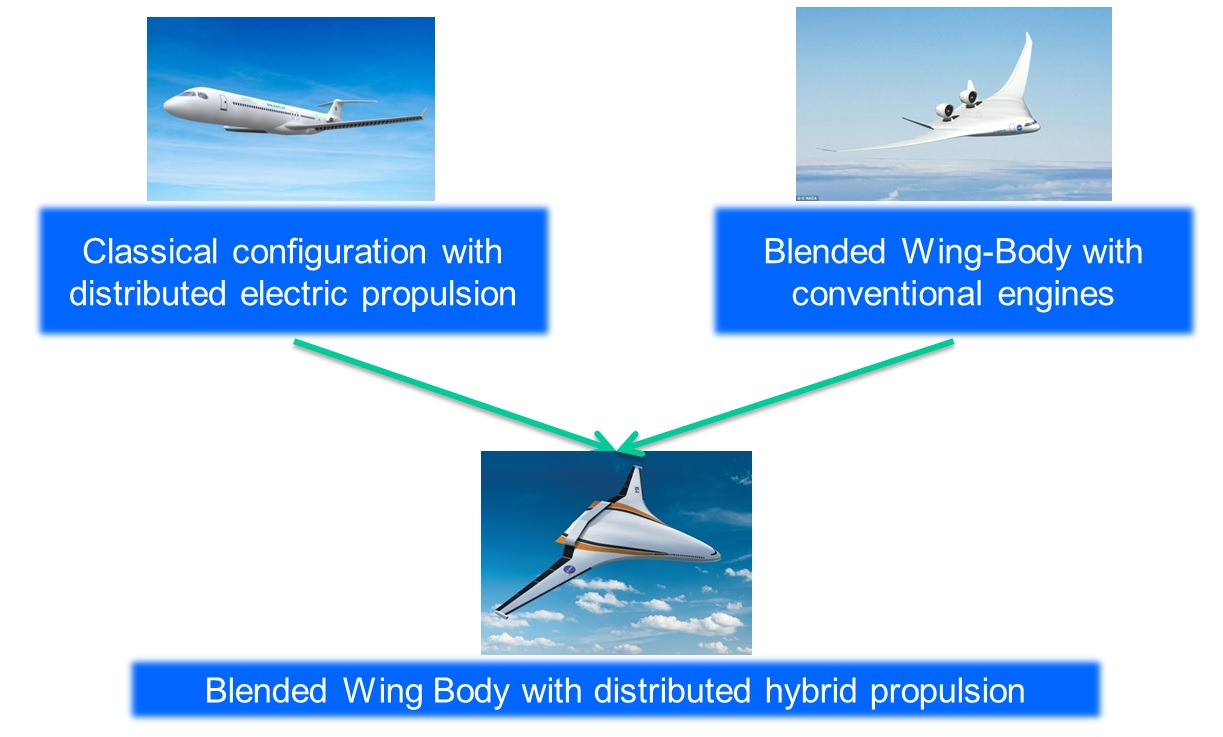
\includegraphics[keepaspectratio, width=\textwidth]{images/chap1/phd_roadmap.jpg}
	\caption{Ph.D. roadmap, representing the two separated steps to finally converge toward the Blended Wing-Body with distributed electric propulsion configuration.}
	\label{fig:phd_roadmap}
\end{figure}

\clearpage

\begin{mdframed}[hidealllines=true,backgroundcolor=blue!20]
	\section*{Synthesis of the chapter}
	
	\begin{itemize}
		\item Increase of emission poses a problem for aviation: to reduce the environmental footprint, a disruptive concept must be introduced. 
		
		\item The exploration of an innovative concept must be carried out at conceptual design level. 
		
		\item Key technologies to match the enviromental goals are explored:
			\begin{itemize}
				
				\item[-] Hybrid and electric propulsion offers new and still unexplored features. 
				
				\item[-] Blended Wing-Body is identified as the most promising architecture for the integration with a distributed electric propulsion system.
				
				\item[-] Blended Wing-Body with distributed electric propulsion is chosen as test case for the research.
				
			\end{itemize}
		
		\item Because of the strong integration among disciplines for unconventional aircraft, classical conceptual design loop based on Multidisciplinary Design Analysis may lead to misleading results: definition of an Overall Aircraft Design procedure based on Multidisciplinary Design Optimisation technique is investigated. 
		
		\item The two key technologies introduced (hybrid propulsion and BWB architecture) are studied separately: final concept results from the merging between the two. 
	\end{itemize}
\end{mdframed}